%======================================================================
%   Zak Webb
%   Ph.D. Thesis
%   Department of Physics and Astronomy
%   University of Waterloo
% 
%   Universality of multi-particle scattering
%======================================================================


\documentclass[../thesis-main/thesis-main]{subfiles}
\begin{document}

\chapter{Universality of multi-particle quantum walk}
\label{chap:MP_universality}

So far in this thesis, we have managed to show several basic results for single-particle scattering on graphs in \chap{scattering_on_graphs} and \chap{scattering_gadgets}, which we then combined in \chap{SP_universality} to show that quantum walk is universal for quantum computing.  We then proved many analogous results for multi-particle quantum walk in \chap{MPQW}, and we might then question whether this system is also universal.  As MPQW is a generalization of quantum walk, we have that this model is already universal for quantum computing from, but this reduction requires the  same exponential sized graph as in \chap{SP_universality}.  The interesting question for MPQW is then whether the model remains universal when we restrict ourselves to polynomially sized graphs.

Without surprising anyone, this chapter is dedicated to proving this universality result.  The proof strategy is very similar to that of \chap{SP_universality}, in that we encode the computational state in a traveling wave-packet, using the ideas of graph scattering in order to implement single-qubit gates.  The difference, however, for the multi-particle case is that we encode each qubit via a different particle, thus allowing for much smaller graphs at the expense of more complicated multi-gate behavior.  In particular, we will implement two-qubit gates using gadgets from \chap{scattering_gadgets} to route two particles toward each other, and then us our results on two-particle scattering from \thm{two_particle_wave-packet_bound} to understand the resulting dynamics.

Note that the proof strategy used in this chapter is identical to that of Childs, Gosset, and Webb's \cite{MPQW}.  In particular, the encoding of individual qubits using distinct particles, the simulation of single-qubit gates via scattering, and the form of the two-qubit gates are all as in their paper.  The difference in results between this chapter and their paper arises from improved technical theorems (namely \thm{single_particle_wavepacket_bound} and \thm{two_particle_wave-packet_bound}), along with some additional scattering gadgets found in \chap{scattering_gadgets}.  

The eventual goal of this chapter is to simulate a given circuit $\mathcal{C}_X = U_{M} U_{M-1}\cdots U_1$ acting on some initial state $\ket{x}$, where each gate $U_i$ comes from some universal gate set and the simulation accepts the state with high probability if and only if the circuit accepts with high probability.  We will first show how to do this for a single gate single-qubit computations in \sec{MP_single_qubit_gate_simulation}, with the extension to multiple gates exactly as in \sec{SP_single_qubit_computations}.  We will then extend this technique to multi-qubit computations in \sec{MP_multi_gate_simulation}.

%%%%%%%%%%%%%%%%%%%%%%%%%%%%%%%%%%%%%%%%%%%%%%%%%%%%%%%%%%%%%%%%%%%%%%%%%%
%  Qubit Encodings
%

\section{Qubit Encoding}\label{sec:MP_qubit_encoding}

As is \chap{SP_universality}, the first step for simulating a given quantum circuit will be to encode the Hilbert space that we want to simulate.  In \chap{SP_universality}, we were able to do this by having a number of infinite paths equal to the dimension of the Hilbert space,  where the encoded state corresponded to the path on which the particle was located.  While this construction works, the fact that the number of paths grows exponentially in the number of encoded qubits makes this impractical for constructing a physical system with a quantum walker.

However, for a bounded number of basis states this construction is simple and technically feasible.  The problem of exponential growth arises from the necessary growth of the Hilbert space when having an unbounded number of qubits, since having a larger number of paths was the only means of adding states to the scattering space.  When we analyze the multi-particle quantum walk, adding additional particles then becomes an avenue for increasing the size of the Hilbert space, and we can avoid this exponential increase in the size of the graph.

As such, our encoding of a single-qubit will be identical to that of \chap{SP_universality}; with some specific momenta chosen $k$, we encoded the value of the qubit in a dual-rail encoding.  The value of the encoded qubit will be $\ket{0}$ if the particle is located along the first (top) path, while the value of the encoded qubit will be $\ket{1}$ if the particle is located along the second (bottom) path.

To expand our encoding to multiple qubits, we then add additional paths, but we also add additional particles.  Namely, for each additional qubit, we add two paths and a single particle with some momentum $k_i$.  Again, for that qubit, the value of the encoded qubit is $\ket{0}$ if the particle is located along the top path, wile the value of the qubit will be $\ket{1}$ if the particle moves along the bottom path.

Note that each qubit has its own momentum: while we could require each particle to be encoded at the same momentum, our eventual construction of a multi-qubit entangling gate requires at least two different momenta.  Because of this, we will label each qubits momentum $k_i$, but we will eventually have that most will be equal to some particular value.  One problem that this will lead to is a possible difference in speeds; given the fact that the momenta is explicitly related to the speed of propagation for a given wave-packet, we will need to ensure that the wave-packets move together through the graph.

With the general idea for the encodings out of the way, we will need to explicitly define our states.  In particular, for each qubit we want to simulate, let us assume that there are two infinite paths, where the vertices are labeled as $(x,z,i)$, for $x\in \ZZ$, $z\in \FF_2$ and $i\in[n]$.  Note that the infinite assumption won't be necessary 

Recall from \chap{SP_universality} and \chap{MPQW} that for a given $\sigma$, cutoff length $L$, and momentum $k$, that we used states of the form
\begin{align}
    \ket{\phi_\mu^{L,\sigma}(k)} = \gamma \sum_{\mu - L}^{\mu + L} e^{ikx} e^{-\frac{(x-\mu)^2}{2\sigma^2}} \ket{x}
\end{align}
as our assumed wave-packets.  We will use similar states for our encoded qubits, where $\sigma$ and $L$ will depend on the overall length of the computation.  Moreover, we will use the same $L$ and $\sigma$ for all of the qubits.

In particular, we will have that a logically encoded basis state $\ket{\mathbf{z}}$ for $\mathbf{z}\in \FF_2^n$ will be encoded in the state
\begin{align}
  \ket{\mathbf{z}}_{\text{log}} &= \gamma^n \bigotimes_{j\in [n]} \sum_{\mu_j-L}^{\mu_j+L} e^{i k_j x} e^{- \frac{(x - \mu_j)^2}{2\sigma^2}} \ket{x,z_j,j},\label{eq:MP_u_logical states}
\end{align}
with the rest of the Hilbert space defined in a linear manner.  Note that each individual qubit has its own momentum $k_i$ and position $\mu_i$, and is supported on disjoint sets of vertices.  Further, we have that the $j$-th particle corresponds to the $j$-th qubit.

If we want to restrict our attention to indistinguishable particles, we can easily change our definition of the logical states.  In particular, we have that in the case of bosonic particles,
\begin{align}
  \ket{\mathbf{z}}_{\text{log}}^{\Sym} &= \frac{\gamma^n}{\sqrt{n!}}\sum_{\pi\in S_n} V_\pi \Bigg[\bigotimes_{j\in [n]} \sum_{\mu_j-L}^{\mu_j+L} e^{i k_j x} e^{- \frac{(x - \mu_j)^2}{2\sigma^2}} \ket{x,z_j,j}\Bigg],
\end{align}
while in the case of fermionic particles,
\begin{align}
  \ket{\mathbf{z}}_{\text{log}}^{\ASym} &= \frac{\gamma^n}{\sqrt{n!}}\sum_{\pi\in S_n} (-1)^{\sign(\pi)}V_\pi \Bigg[\bigotimes_{j\in [n]} \sum_{\mu_j-L}^{\mu_j+L} e^{i k_j x} e^{- \frac{(x - \mu_j)^2}{2\sigma^2}} \ket{x,z_j,j}\Bigg].
\end{align}
For the purposes of this chapter, we will usually not care about the symmetries of the particles, as the only time we will use them is in the analysis of the two-particle gadget.  Namely, the phase acquired when two particles move past each other on a long path depends on the symmetries between the particle, and thus the resulting two-qubit unitary will depend on the type of particles.  However, since this chapter is a general construction, the particular two-qubit gate applied does not greatly affect our proof.


%%%%%%%%%%%%%%%%%%%%%%%%%%%%%%%%%%%%%%%
\section{Single-qubit gate simulation}\label{sec:MP_single_qubit_gate_simulation}

With our encoding of the relevant Hilbert space, the next step in our attempt to simulate a given circuit will be to encode the simulation of a single-qubit gate. If we restrict ourselves to a single qubit, this will be done exactly as in \sec{SP_1_single_qubit_unitary}, as our encoded systems are exactly the same.  Namely, for a given qubit with momentum $k$, if we want to apply the unitary $U$, we will place a graph $\widehat{G}$ as an obstacle along the pair of infinite paths, where the scattering matrix at $k$ of $\widehat{G}$ takes the form
\begin{align}
  S(k) = \begin{pmatrix}
    0& U^T\\
    U & 0
  \end{pmatrix},\label{eq:MP_unitary_s_matrix}
\end{align}
and where we assume that the labeling of the four terminal vertices proceeds as $0_{\text{in}}$, $1_{\text{in}}$, $0_{\text{out}}$, and $1_{\text{out}}$, as in \fig{single_qubit_scattering_graph}. 

When we add additional qubits, however, things differ from the single-particle case.  In \chap{SP_universality}, our simulation of a single-qubit unitary on $n$ qubits required $2^{n-1}$ copies of the graph gadget $\widehat{G}$ in order to implement the logical gate, corresponding to the computational basis states of all the qubits that the particular unitary does not effect.  For our multi-particle encoding, only a single copy of the graph is used, and it is placed as an obstacle on the pair of paths corresponding to the qubit on which the gate is to be applied, while the rest of the qubits simply remain unimpeded.  

Assuming that the graph $G$ we use to simulate is of this form, and if the qubits are encoded as in \sec{MP_qubit_encoding} with momenta traveling towards the gadget $\widehat{G}$, we can use \lem{disconnected_MPQW} and \thm{single_particle_wavepacket_bound} to see that the time-evolved state corresponds to the encoded logical state after the unitary $U$ is applied to the appropriate question (modulo some error and details about the encoded logical state at different times).  The intuitive idea behind this scattering behavior is represented schematically in \todo{find fig}.

\subsection{Finite graphs for single-qubit gates}

While an understanding of the scattering behavior for infinite graphs is useful to give a broad overview of the dynamics, we will eventually need to restrict ourselves to finite sized graphs.  In particular, we will restrict ourselves exactly as in the case for single-particle scattering in \chap{SP_universality}.  Moreover, we will actually be able to use \lem{single_qubit_encoded_computation}, as our encoded logical states satisfy the assumptions of \lem{disconnected_MPQW}.  More exactly, we will be able to use \lem{disconnected_MPQW} to evolve each particle independently of the others using the approximations of \lem{single_qubit_encoded_computation}, and see that the errors add linearly.

\begin{figure}
  \centering  
  \tikzsetnextfilename{MP_u_sqf}
  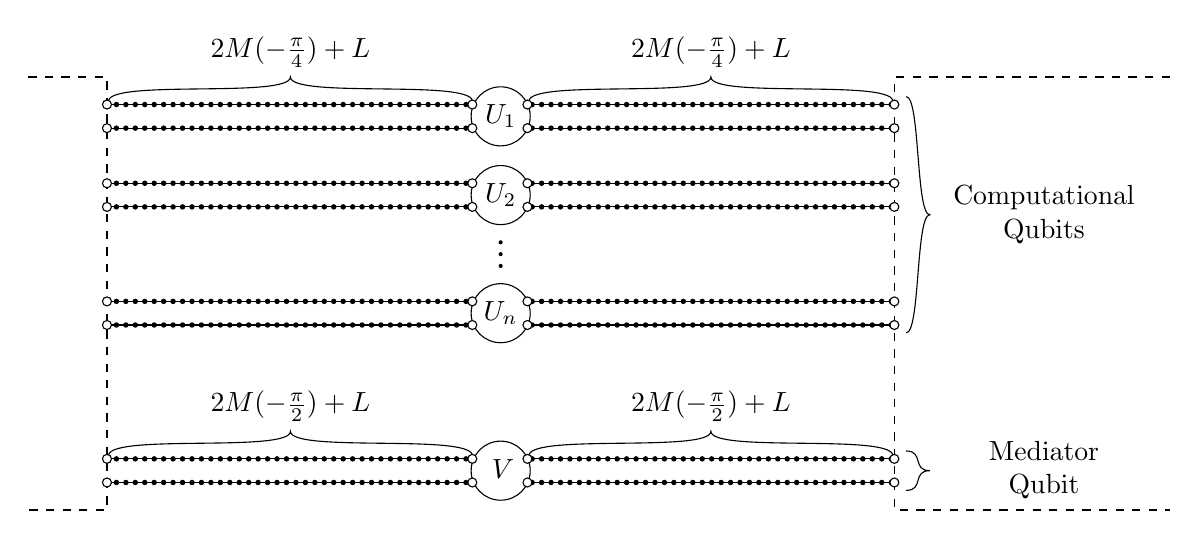
\begin{tikzpicture}[
  unitary/.style={circle,draw=black,fill=white,
    inner sep=0pt,minimum size=7.5mm},
  dots/.style={circle,fill=black,
    inner sep=0pt,minimum size=1.5pt},
  vert/.style={circle,fill=black,
    inner sep=.7pt,minimum size=0pt},
  attach/.style={circle,draw=black,fill=white,inner sep=1.15pt,minimum size=0}]

  \foreach \n /\y in {U_1/2.5,U_2/1.5,U_n/0,{V_{\med}}/-2}{
    \begin{scope}[yshift = \y cm]
      \foreach \x in {0,.12,...,10} {
        \node at (\x, -.15) [vert] {};
        \node at (\x, .15) [vert] {};
      }
      \draw (0, -.15) to (10, -.15);
      \draw (0,  .15) to (10,  .15);
      \node at (5,0) [unitary]{$ \n $};


    \end{scope}
  }
  
  \foreach \x in {0,5.34}{
  \foreach \y /\p in {2.5/4,-2/2}{
  \begin{scope}[xshift=\x cm,yshift=\y cm]
    \node (\x\p) at (2.33,.5)[above] {$2M(-\frac{\pi}{\p}) + L$};
  
    \draw (0.02,0.2) to[out=80,in=-90,looseness=0.3] (2.33,.5)
                     to[out=-90,in=100,looseness=0.3] (4.64,.2);
  \end{scope}}} 
                  
  \draw (10.15,2.75) to[out=0,in=-180,looseness=0.3] (10.45,1.25)
                    to[out=-180,in=0,looseness=0.3] (10.15,-.25);
  \node at (11.9,1.25)
      {\begin{tabular}{c}
          Computational\\ 
          Qubits\end{tabular}};


  \draw (-1,3) to (0, 3) to (0,-2.5) to (-1,-2.5) [dashed];
  \draw (13.5,3) to (10,3) to (10,-2.5) to (13.5,-2.5) [dashed];

  \node at (5,.9) [dots] {};
  \node at (5,.75)    [dots] {};
  \node at (5,.6) [dots] {};

  \draw (10.15,-1.75) to[out=0,in=-180,looseness=1.5] (10.45,-2)
                    to[out=-180,in=0,looseness=1.5] (10.15,-2.25);
  \node at (11.9,-2) 
      {\begin{tabular}{c}
          Mediator\\ 
          Qubit\end{tabular}};
          
   \foreach \x in {0, 10, 4.64, 5.34}{
   \foreach \y in {2.35,2.65,1.65,1.35,.15,-.15,-1.85,-2.15}{
     \node at (\x, \y) [attach] {};
   }}
\end{tikzpicture}
  \caption[MPQW single-qubit unitary]{A finite graph applying a single-qubit unitary to the first qubit.}
\label{fig:MP_u_sqf}
\end{figure}


Along these lines, let us assume that we want to apply a single-qubit gate $U$ to qubit $j$, where there exists a gadget $\widehat{G}$ that implements this unitary at momentum $k_j$.  We then let $H = A(G)$, where $G$ is the infinite graph corresponding to single-particle scattering off of $\widehat{G}$ along with $2(n-1)$ infinite paths.  Let $G(\vec{K})$ then be the finite graph obtained from $G$, where we truncate each semi-infinite path attached to $\widehat{G}$ to total length $K_j$, and we truncate the infinite paths so that there are two length-$(2K_\ell+2)$ paths for each $\ell\in [n]$ with $\ell\neq j$.  We have that the vertices on the long paths are labeled by $(\ell,z,x)$ for $j\neq\ell\in [n]$ $z\in \FF_2$ and $x\in \ZZ$ with $|x| \leq K_\ell$, while the vertices on the paths connected to $\widehat{G}$ are labeled $(j,x,i)$ for $1\leq x \leq K_j$, $i\in [4]$ (as in \sec{SP_single_qubit_finite_graph}).  Let the subspace $\mathcal{K}$ be spanned by basis states corresponding to vertices in $G(K)$.  Graphs of this form will be used to simulate the application of $U$ to qubit $j$.

We show that for specific $\mu_\ell$, $\sigma$, $L$, and $\vec{K}$, initial logical states evolve to output logical states.  In particular, let us assume that the $j$-th particle is in the state
\begin{align}
  \ket{z}_{\text{log},\text{in},j} = \gamma \sum_{x = \mu_j - L}^{\mu_j + L} e^{ i k_j x} e^{ - \frac{(x-\mu_j)^2}{2\sigma^2}} \ket{j,x,z},
  \label{eq:single_qubit_important_state_in}
\end{align}
while each of the other particles are in the state
\begin{align}
  \ket{z}_{\text{log},\text{in},\ell} = \gamma \sum_{x = -\mu_\ell-L}^{-\mu_\ell + L} e^{- i k_\ell x} e^{ - \frac{(x-\mu_\ell)^2}{2\sigma^2}} \ket{\ell,x,z+1}.
\end{align}
Further, let us assume that each $\mu_\ell = T \sin |k_\ell|$, so that each particle travels a distance $2 \mu_\ell$ in time $T$.  We then have that after a time $T$, we will want the output logical states to be given by 
\begin{align}
  \ket{z}_{\text{log},\text{out},j} = \gamma e^{-2iT \cos(k_j)}\sum_{x = \mu_j - L}^{\mu_j + L} e^{- i k_j x} e^{ - \frac{(x-\mu_j)^2}{2\sigma^2}} \ket{j,x,z+3},
  \label{eq:single_qubit_important_state_out}
\end{align}
for the $j$-th particle, while each of the other particles are in the state
\begin{align}
  \ket{z}_{\text{log},\text{out},\ell} = \gamma e^{-2i T \cos(k_\ell)} \sum_{x = \mu_\ell-L}^{\mu_\ell + L} e^{- i k_\ell x} e^{ - \frac{(x-\mu_\ell)^2}{2\sigma^2}} \ket{\ell,x,z}.
\end{align}
As in the case for single-particle universality, for a give state $\ket{\phi} = \sum_{x\in \FF_2^n} \alpha_x \ket{x}$, we define the encoded state
\begin{align}
  \ket{\phi}_{\text{log,in}} = \sum_{x\in \FF_2^n} \alpha_{x} \bigotimes_{i=1}^n \ket{x_i}_{\text{log},\text{in,i}}\label{eq:MP_single_input_encoding}
\end{align}
and for a given unitary $U$,
\begin{align}
  \ket{U\phi}_{\text{log,out}} = \sum_{x,y\in \FF_2^n} U_{xy}\alpha_{y} \bigotimes_{i=1}^n \ket{x_i}_{\text{log},\text{in,i}}.\label{eq:MP_single_output_encoding}
\end{align}

With these definitions, we can give an analogous result to \lem{single_qubit_encoded_computation}.

\begin{lemma}
\label{lem:MP_u_single_qubit_encoded_computation}
  Let $k_j\in (-\pi,0)$ for all $j\in [n]$, and let $\widehat{G}$ be a four-terminal gate gadget, such that its scattering matrix at momentum $k_j$ is of the form \eq{MP_unitary_s_matrix}.  Letting the logical states $\ket{z}_{\text{log},\text{in}}$ and $\ket{z}_{\text{log},\text{out}}$ be defined as in \eq{MP_single_input_encoding} and \eq{MP_single_output_encoding}, and let $G(K)$ be defined as above, where each $\mu_\ell \geq L $, $K_\ell \geq \frac{5 \mu_\ell}{3}$, and $T = \frac{\mu_\ell}{\sin |k_\ell|}$, we have that there exists some constant $\xi$ such that for all $0 \leq t \leq T$ and any interaction $\mathcal{U}$,
\begin{align}
  \Big\Vert e^{-i H_G^N t} \ket{\phi(0)} - \ket{\phi(t)} \Big\Vert \leq \xi n \sqrt{\frac{\log L}{L}},
\end{align}
where
\begin{align}
  \ket{\phi(t)} = \sum_{x\in\FF_2^n} \alpha_x \bigotimes_{\ell=1}^n   \ket{\alpha^{x_\ell}_\ell(t)},
\end{align}
the $\ket{\alpha^{x_j}_j(t)}$ are equal to $\ket{\alpha^1(t)}$ and $\ket{\alpha^2(t)}$ as defined in \thm{single_particle_wavepacket_bound}, and for the rest of the particles we have
\begin{align}
  \ket{\alpha_\ell^z(t)} = \gamma e^{-2it \cos (k_\ell)} \sum_{x = \mu_\ell(t)-L}^{\mu_\ell(t) + L} e^{- i k_\ell x} e^{ - \frac{(x-\mu_\ell(t))^2}{2\sigma^2}} \ket{\ell,x,z},
\end{align}
with
\begin{align}
  \mu_\ell(t) &= -\mu_\ell + 2t \sin |k_\ell|.
\end{align}
In particular, we have
\begin{align}
  \Big\Vert e^{-i H_G^N T} \ket{\psi}_{\text{log},\text{in}} - \ket{U\psi}_{\text{log},\text{out}}\Big\Vert \leq \xi n\sqrt{\frac{\log L}{L}}.
\end{align}
\end{lemma}

\begin{proof}
  Note that the states $\ket{\phi(t)}$ all have the particles supported on different components of $G$, and thus by \lem{disconnected_MPQW} we have that
  \begin{align}
    e^{-i H_G^N t} \ket{\phi(0)} &= \prod_{\ell=1}^n \big( e^{-i A(G_\ell)t}\big)^{(\ell)} \ket{phi(0)},
  \end{align}
where $G_\ell$ is the component on which the $\ell$-th particle is located.  However, we have that each of these unitaries commute, and
  \begin{align}
    \big( e^{-i A(G_\ell)t}\big)^{(\ell)} \ket{\phi(0)}&= \sum_{x\in \FF_2^n} \alpha_x \bigotimes_{i=1}^n e^{- i \delta_{i,\ell} A(G_\ell) t} \ket{\alpha_i^{x_i}(0)}\\
    & = \sum_{x\in \FF_2^n} \alpha_x \Bigg[\bigotimes_{i=1}^n \Big(\ket{\alpha_i^{x_i}(\delta_{\ell,i} t)} + \delta_{\ell,i} \ket{\epsilon_{\alpha_x,\ell}(t)}\Big)\Bigg],
  \end{align}
  by \lem{single_qubit_encoded_computation}, with $\Vert \ket{\epsilon_{\alpha_x,\ell}(t)}\Vert \leq \xi \sqrt{\log L/L}$ for some constant $\xi$.  (We can use the theorem to understand the scattering on the paths, with $\widehat{G}$ the four-terminal gadget composed of two length-2 paths in the middle of the length $2K_i + 2$ length paths.)
  
  Combining these results, we then have that
  \begin{align}
    e^{-i H_G^N t} \ket{\phi(0)} &= \sum_{x\in \FF_2^n} \alpha_x \Bigg[\bigotimes_{i=1}^n \Big(\ket{\alpha_i^{x_i}(t)} + \ket{\epsilon_{\alpha_x,\ell}(t)}\Big)\Bigg]\\
      &= \ket{\phi(t)} + \ket{\varepsilon(t)},
  \end{align}
  where $\Vert \ket{\varepsilon(t)}\Vert \leq n \xi \sqrt{\log L/L}$.

\end{proof}

Note that most of the analysis up until this point is essentially a rehashing of results from \chap{SP_universality}, as we have kept the particles far apart. 




%%%%%%%%%%%%%%%%%%%%%%%%%%%%%%%%%%%%%%%%%%%%%%%%%%%%%%%%%%%%%%%%%%%%%%%%%%
%  Applying an encoded C\theta gate
%

\section{Entangling gate}\label{sec:entangling_gate}


Now that we have encoded qubits and, at specific momenta, a universal set of single-qubit gates, we need to construct some kind of entangling gate between our encoded qubits.  In the single-particle encoding, this gate was trivial, as a controlled-not gate (and in fact any permutation gate) simply corresponded to a relabelling of the encoding paths.  For our multi-particle encoding, however, the entanglement procedure is rather more involved.  Our gate will necessarily involve a two-particle Hamiltonian, but we will arrange the graph (and the encoded states) in such a manner that the two-particles will only ever interact on a (long) path.  As such, we can use \thm{two_particle_wave-packet_bound} to see that the result of such scattering is simply an applied phase (at least when particles are indistinguishable).

Explicitly, our entangling gate will be a controlled-$\theta$ gate, for some $\theta$ that depends on the interaction and the momenta used to encode the qubits.  Further, our entangling gate will only exist between qubits that are encoded with particles for which a momentum switch (see \sec{mom_switch}) exists, which necessitates the use of at least two different momenta.  The main idea behind the gate is to place two momentum switches (represented schematically as \fig{mom_switch}) on the $1$-paths of the qubits as obstacles, where the two switches are connected by a long path for their third terminals.  If either particle is in the logical state $1$, it will be routed along the long connecting path between the two paths, and then routed along $1_{\text{out}}$ for the opposite qubit.  By arranging the lengths of the various paths correctly, we can ensure that if at most a single encoded qubit is in the logical $1$ state, then the corresponding single-particle scattering events encode identity operations.  However, if both encoded qubits are logically $1$, then the two particles move past each other along the long connecting path, acquiring an additional phase that depends on their momenta and the interaction.  As such, the graph in \fig{cd_gate} applies an encoded $\CD$ gate (along two single-qubit gates arising from the phase acquired during the momentum switches).

Note that the graph and analysis described here only works for two particles.  However, we will use a lemma similar to \lem{MP_u_single_qubit_encoded_computation} in order to analyze the related $n$-particle Hamiltonian.

\begin{figure}
\centering
\subfloat[][]{
  \tikzsetnextfilename{MP_u_mom_switch}
  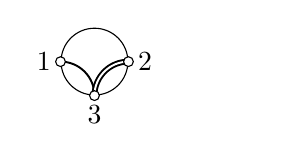
\begin{tikzpicture}
  [ scale = 0.6,
    thin,
    inner/.style={circle,draw=black!100,fill=black!100,inner sep=1.25pt},
    attach/.style={circle,draw=black!100,fill=black!0,thin,inner sep=1.25pt},
    sin/.style={line width=.7pt},
    doub/.style={line width=2.1pt},
    trip/.style={draw=white,line width=.7pt}]
    \node at (0,0){};
%\begin{scope}[yshift=1.8cm]
%  \node (2)  at (0,0) [attach,label=left:3] {};
%  \node (1)  at (0,1) [attach,label=left:1] {};
%  \node (3)  at (3,1) [attach,label=right:2] {};
%  \node (4)  at (1,0) [inner]  {};
%  \node (5)  at (2,0) [inner]  {};
%  \node (6)  at (1,1) [inner]  {};
%  \node (7)  at (2,1) [inner]  {};
%  \node (8)  at (2,2) [inner]  {};
%  \node (9)  at (2.866,2.5)  [inner] {};
%  \node (10) at (1.134,2.5)  [inner] {};
%  \node (11) at (2,-1)       [inner] {};
%  \node (12) at (2.866,-1.5) [inner] {};
%  \node (13) at (1.134,-1.5) [inner] {};
%
%  \draw (2) to (4);
%  \draw (4) to (5);
%  \draw (3) to (7);
%  \draw (1) to (6);
%  \draw (6) to (4);
%  \draw (6) to (7);
%  \draw (7) to (5);
%  \draw (7) to (8);
%  \draw (8) to (9);
%  \draw (8) to (10);
%  \draw (11) to (5);
%  \draw (11) to (12);
%  \draw (11) to (13);
%
  \node (split) at (-3.6,.8) [draw=black,circle,inner sep=3mm,
         label=left:1,label=right:2,label=below:3] {};
% 
%  \node at (-1.6,.5) {=};

  \draw[sin]  (split.west) to[out=0,in=90]   (split.south);
  \draw[doub] (split.east) to[out=180,in=90] (split.south);
  \draw[trip] (split.east) to[out=180,in=90] (split.south);
  
  \node at (split.east) [attach] {};
  \node at (split.west) [attach] {};
  \node at (split.south) [attach]{};
%\end{scope}
\end{tikzpicture}
  \label{fig:mom_switch}
}
\hspace{0.5cm}
\subfloat[][]{
  \tikzsetnextfilename{MP_u_cd_gate}
  \begin{tikzpicture}
  [ scale = 1,
    yscale = .8,
    attach/.style={circle,draw=black!100,fill=white,thick,
    minimum size = 6mm},
    cross/.style={line width=4pt, draw=white},
    drawn/.style={draw=black},
    vert/.style = {circle,fill=black,inner sep=.6pt, minimum size=0},
    nofill/.style = {circle,draw=black,fill=white,inner sep = 1.25pt,minimum size=0},
    decoration={markings,
		mark=between positions 0 and 10 step .1cm
 		with { \node at (0,0) [vert]{}; }}]

  \node (bottom) at ( 1, 0) [attach] {};
  \node (top)    at ( 1, 2.5) [attach] {};
  
  \foreach \x in {0,.1,...,3.5}{
  \foreach \y in {.75, 3.25}{
    \node at (\x,\y) [vert] {};
  }}

  \draw[postaction={decorate}] (0,0) node[left] {$1_{\med,\text{in}}$} 
    -- (bottom.west);
  \draw (0,.75) node [left] {$0_{\med,\text{in}}$} 
    -- (3.5,.75) node [right] {$0_{\med,\text{out}}$};
  \draw (0,3.25) node [left] {$0_{c,\text{in}}$}
    -- (3.5,3.25) node [right] {$0_{c,\text{out}}$};
  \draw[postaction={decorate}] (0,2.5) node [left] {$1_{c,\text{in}}$} 
    -- (top.west) ;
  \draw (top.south) -- (bottom.north) [cross];

  \draw (top.south) -- (bottom.north) [drawn,postaction={decorate}];
  \draw (top.east) -- ( 2, 2.5)  .. controls (2.5,2.5) and (2.5, 0) 
                   .. (3,0) -- (3.5, 0)  [cross];
  \draw (top.east) -- ( 2, 2.5)  .. controls (2.5,2.5) and (2.5, 0) 
                    .. (3,0) -- (3.5, 0) 
                    node [right] {$1_{\med,\text{out}}$} [drawn,postaction={decorate}];
  \draw (bottom.east) -- ( 2, 0) .. controls (2.5,0) and (2.5,2.5)  
                      .. (3,2.5) -- (3.5, 2.5)  [cross];
  \draw[drawn,postaction={decorate}] (bottom.east) -- ( 2, 0) .. controls (2.5,0) and (2.5,2.5)  
                      .. (3,2.5) -- (3.5, 2.5) 
                      node [right] {$1_{c,\text{out}}$} ;

  \draw (top.west) to[out=0,in=90] (top.south) [line width = .7pt];
  \draw (bottom.east) to[out=-180,in=-90] (bottom.north) [line width=.7pt];
  \draw (top.east) to[out=-180,in=90] (top.south) [line width=2.1pt];
  \draw (top.east) to[out=-180,in=90] (top.south) [line width=.7pt,draw=white];
  \draw (bottom.west) to[out=0,in=-90] (bottom.north) [line width=2.1pt];
  \draw (bottom.west) to[out=0,in=-90] (bottom.north) [line width=.7pt,draw=white];  
  
  
  \foreach \x in {0, 3.5}{
  \foreach \y in {0,.75, 2.5, 3.25}{
    \node at (\x,\y) [nofill] {};
  }}
 
 \node at (top.west) [nofill]{};
 \node at (top.east) [nofill]{};
 \node at (top.south) [nofill]{};
 \node at (bottom.west) [nofill]{};
 \node at (bottom.east) [nofill]{};
 \node at (bottom.north) [nofill]{};
  
\end{tikzpicture}
  \label{fig:cd_gate}
}
\caption[MPQW $\CD$ gate]{\subfig{mom_switch} Momentum switch schematic. \subfig{cd_gate} $\CD$ gate.}
\label{fig:onepsplit}
\end{figure}

\subsubsection{Momentum switch}

Remember from \sec{mom_switch} that momentum switches are three-terminal scattering gadgets that act like railroad switches, where at specific momenta the gadget has perfect transmission from terminal 3 to terminal 1, while at other momenta there is perfect transmission from terminal 3 to terminal 2.  We will represent gadgets with this behavior schematically as in \fig{mom_switch}, where one set of momenta follow the single line while the other specified set follows the double line.

For our purposes, we will assume that the momentum switch splits the two momenta used to encode the different qubits $k_{1}$ and $k_{2}$.  Explicitly, we will assume that the $S$-matrix for the given momentum switch at $k_1$ and $k_2$ are given by
\begin{equation}
  S_{\text{switch}}(k_{1}) = \begin{pmatrix} 0 & 0 & T_{1}\\
    0 & R_{1} & 0\\
    T_{1} & 0 & 0\end{pmatrix}\qquad
  S_{\text{switch}}(k_{2}) = \begin{pmatrix}R_{2} & 0 &0\\
    0 & 0 & T_{2}\\
    0 & T_{2} & 0\end{pmatrix}.
\label{eq:switch_S}
\end{equation}
In other words, we will assume that the momentum switch has perfect transmission between terminals $1$ and $3$ at momentum $k_{1}$, and perfect transmission between terminals $2$ and $3$ at momentum $k_{2}$, possibly with an additional phase.  With this, we have that a particle with momentum $k_{1}$ follows the single line of the schematic representation of \fig{mom_switch}, while a particle with momentum $k_{2}$ follows the double line.


\subsection{Constructing the graph}

We will now construct the entangling graph, where we will assume that we know the encoded initial states.  Note that this construction depends on the momenta of the encoded qubits in more than just the form of the momentum switch; the fact that the timing of the wave-packets is important forces us to change the length of the connecting paths depending on the initial momentum so that they arrive on the infinite path at the same time, while the requirement that the particles only interact along the path forces us to change the lengths depending on the size of the wave-packets.

The $\CD$ gate is implemented using the graph shown in \fig{explicit_cd}. In this section we specify the logical input states, the logical output states, the distances $X$, $Z$, and $W$ appearing in the figure, and the total evolution time as functions of the momentum $k_{1}$ and $k_{2}$. With these choices, we show that a $\CD$ gate is applied to the logical states at the end of the time evolution under the quantum walk Hamiltonian (up to error terms that are $\tilde{\OO}(L^{-{1}/{2}})$). The results of this section pertain to the two-particle Hamiltonian $H^{(2)}_{G'}$ for the graph $G'$ shown in \fig{explicit_cd}.

\begin{figure}
  \centering
  \tikzsetnextfilename{MP_u_explicit_cd}
  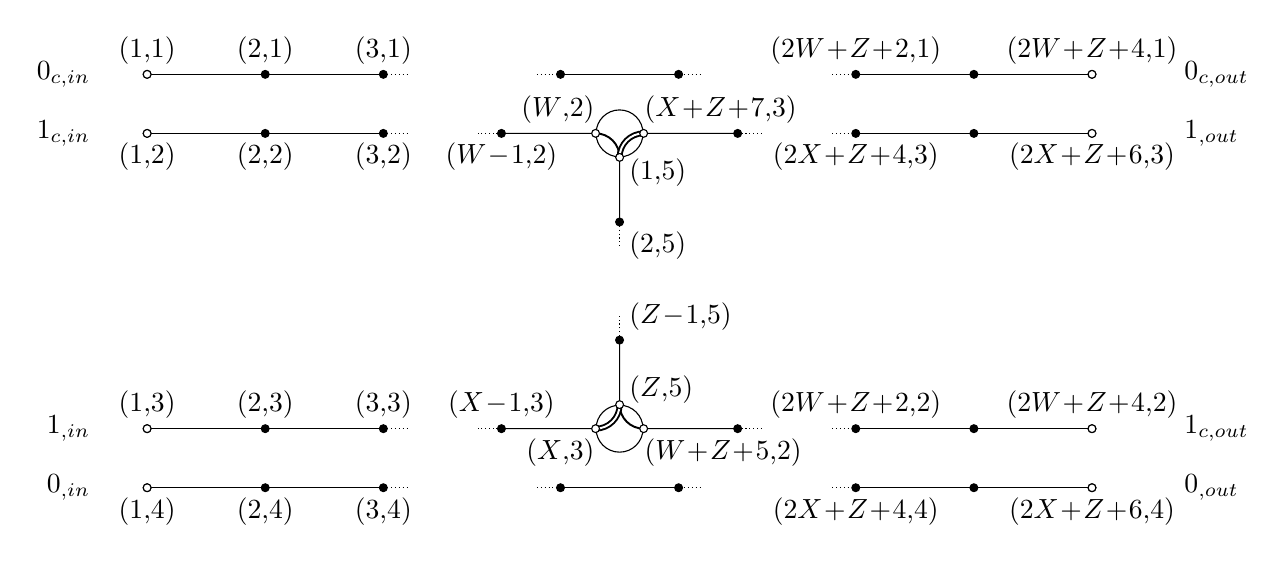
\begin{tikzpicture} [scale=1.5,
	vert/.style={circle, draw=black, fill=black,inner sep=1pt, minimum width=0pt},
	dots/.style={circle, fill=black,inner sep=1pt, minimum width=0pt},
	switch/.style={circle,draw=black,inner sep=6pt,minimum width=0pt},
	attach/.style={circle,fill=white, draw=black,inner sep=1pt, minimum width=0pt}]

  \foreach \y in {0,0.5,3,3.5}{
  \begin{scope}[yshift=\y cm]
  \foreach \x in {0,1,2,6,7,8}{
	\begin{scope}[xshift = \x cm]
	  \node at (0,0) [vert]{};
	\end{scope}}
	\draw (0,0) -- (2,0);
	\draw (6,0) -- (8,0);
	\draw[densely dotted] (2,0)--(2.2,0);
	\draw[densely dotted] (5.8,0)--(6,0);
	\node at (0,0) [attach] {};
	\node at (8,0) [attach] {};
 \end{scope}}
 
  
  \node (switch2) at (4,0.5)[switch]{};
  \node (switch1) at (4,3)[switch]{};
  
  \node at (3,0.5) [vert]{};
  \node at (3,3) [vert]{};
  \node at (5,0.5) [vert]{};
  \node at (5,3) [vert]{};
  
  \draw (switch2.west) -- (3,0.5);
  \draw[densely dotted] (3,0.5) -- (2.8,0.5);
  \draw (switch2.east) -- (5,0.5);
  \draw[densely dotted] (5,0.5) -- (5.2,0.5);
  
  \draw (switch1.west) -- (3,3);
  \draw[densely dotted] (3,3) -- (2.8,3);
  \draw (switch1.east) -- (5,3);
  \draw[densely dotted] (5,3) -- (5.2,3);
  
  \node at (3.5,0) [vert]{};
  \node at (4.5,0) [vert]{};
  \node at (3.5,3.5) [vert]{};
  \node at (4.5,3.5) [vert]{};
  
  \draw (3.5,0) -- (4.5,0);
  \draw (3.5,3.5) -- (4.5,3.5);
  \draw[densely dotted] (3.3,0) -- (4.7,0);
  \draw[densely dotted] (3.3,3.5) -- (4.7,3.5);
  

  \node at (4,1.25) [vert] {};
  \node at (4,2.25) [vert] {};
  
  \draw (switch2.north) -- (4,1.25);
  \draw[densely dotted] (4,1.25) -- (4,1.45);
  
  \draw (switch1.south) -- (4,2.25);
  \draw[densely dotted] (4,2.25)-- (4,2.05);
  
  \draw[line width=.7pt] (switch1.west) to[out=0,in=90] (switch1.south);
  \draw[line width=2.1pt] (switch1.east) to[out=180,in=90] (switch1.south);
  \draw[line width=.7pt,white] (switch1.east) to[out=180,in=90] (switch1.south);

  \draw[line width=.7pt] (switch2.east) to[out=180,in=-90] (switch2.north);
  \draw[line width=2.1pt] (switch2.west) to[out=0,in=-90] (switch2.north);
  \draw[line width=.7pt,white] (switch2.west) to[out=0,in=-90] (switch2.north);
  
  \node at (switch2.north) [attach] {};
  \node at (switch1.south) [attach] {};
  \node at (switch2.east) [attach] {};
  \node at (switch1.east) [attach] {};
  \node at (switch2.west) [attach] {};
  \node at (switch1.west) [attach] {};
  
  \node at (0,0) [below] {(1,4)};
  \node at (1,0) [below] {(2,4)};
  \node at (2,0) [below] {(3,4)};
  \node at (3.5,0) [below] {};
  \node at (4.5,0) [below] {};
  \node at (6,0) [below] {($2X\!+\! Z\! + \! 4$,4)};
  \node at (8,0) [below] {($2X\! +\! Z\! +\! 6$,4)};
  
  \node at (0,3.5) [above] {(1,1)};
  \node at (1,3.5) [above] {(2,1)};
  \node at (2,3.5) [above] {(3,1)};
  \node at (3.5,3.5) [above] {};
  \node at (4.5,3.5) [above] {};
  \node at (6,3.5) [above] {($2W\! + \! Z\! + \! 2$,1)};
  \node at (8,3.5) [above] {($2W\! + \! Z\! + \! 4$,1)};
  
  \node at (0,3) [below] {(1,2)};
  \node at (1,3) [below] {(2,2)};
  \node at (2,3) [below] {(3,2)};
  \node at (3,3) [below] {($W\!-\! 1$,2)};
  \node[anchor=south east] at (3.87,3) {($W$,2)};
  
  \node at (0,.5) [above] {(1,3)};
  \node at (1,.5) [above] {(2,3)};
  \node at (2,.5) [above] {(3,3)};
  \node at (3,.5) [above] {($X\! -\! 1$,3)};
  \node at (3.87,.5) [below left] {($X$,3)};
  
  \node at (8,.5) [above] {($2W\! + \! Z\! + \! 4$,2)};
  \node at (6,.5) [above] {($2W\! + \! Z\! + \! 2$,2)};
  \node at (4.13,.5) [below right] {($W\! + \! Z\! + \! 5$,2)};  
  
  \node at (8,3) [below] {($2X\! + \! Z\! + \! 6$,3)};
  \node at (6,3) [below] {($2X\! + \! Z\! + \! 4$,3)};
  \node at (4.13,3) [above right] {($X\! + \! Z\! + \! 7$,3)};
  
  \node at (4,2.87) [below right] {(1,5)};
  \node at (4,2.25) [below right] {(2,5)};
  
  \node at (4,.63) [above right] {($Z$,5)};
  \node at (4,1.25) [above right] {($Z\! -\! 1$,5)};
  
  \node at (-.4,0) [left] {$0_{\med,\text{in}}$};
  \node at (-.4,.5) [left] {$1_{\med,\text{in}}$};
  \node at (-.4,3) [left] {$1_{c,\text{in}}$};
  \node at (-.4,3.5) [left] {$0_{c,\text{in}}$};
  
  \node at (8.7,0) [right] {$0_{\med,\text{out}}$};
  \node at (8.7,.5) [right] {$1_{c,\text{out}}$};
  \node at (8.7,3) [right] {$1_{\med,\text{out}}$};
  \node at (8.7,3.5) [right] {$0_{c,\text{out}}$};
\end{tikzpicture} 
  \caption[Explicit $\CD$ gate]{Graph $G'$ used to implement the $\CD$ gate. The integers $Z$, $X$, and $W$ are specified in equations \eq{Z_eq}, \eq{X_eq}, and \eq{W_eq}, respectively.}
\label{fig:explicit_cd}
\end{figure}

We first need to construct the assumed encoded initial states.  Note that the important feature about these encodings are the momenta $k_i$ and  the cutoff distance $L$.  While the distance from the ends and the distance from the scattering widgets are important, they won't affect the overall qualitative action of the wave-packets.  With the labelling scheme for the vertices as in \fig{explicit_cd}, we can then assume that our initial logical states are
\begin{align}
  |0_{\text{in}}\rangle^{1}&=  \gamma \sum_{x = \mu_1 -L} ^{\mu_1 + L}  e^{i k_{1} x} e^{- \frac{(x-\mu_1)^2}{2\sigma^2}} \ket{x,1} & 
  |1_\text{in}\rangle^1&= \gamma \sum_{x = \mu_1 -L} ^{\mu_1 + L}  e^{i k_{1} x} e^{- \frac{(x-\mu_1)^2}{2\sigma^2}} \ket{x,2} \label{eq:cd_input_1}
\end{align}
for the qubit with momentum $k_1$ and
\begin{align}
  |0_{\text{in}}\rangle^2&=\gamma \sum_{x = \mu_2 -L} ^{\mu_2 + L}  e^{i k_{2} x} e^{- \frac{(x-\mu_2)^2}{2\sigma^2}} \ket{x,4}&
  |1_\text{in}\rangle^2&=\gamma \sum_{x = \mu_2 -L} ^{\mu_2 + L}  e^{i k_{2} x} e^{- \frac{(x-\mu_2)^2}{2\sigma^2}} \ket{x,3} \label{eq:cd_input_2}
\end{align}
 for the qubit with momentum $k_2$.  Additionally, let us assume that $|\sin k_1| \leq |\sin k_2|$, so that the wave-packet with momentum $k_1$ travels no faster than the wave-packet with momentum $k_2$ (this assumption is without loss of generality as we can simply relabel $k_1$ and $k_2$).
 
 Note that the two computational basis states for each qubit are centered at the same distance from the ends, but that the distances are different for the two qubits.  The reason for this is that while the wave-packets for each individual qubit travel at the same speed, the fact that $k_1\neq k_2$ (which is implied by the existence of the momentum switch) allows the two wave-packets to travel at differing speeds.  This difference in the distance allows us to ensure that this difference in speed is taken care of when we combine these gadgets.
 
With these initial logical states chosen, note that there are seven path lengths that we will need to determine before we can analyze the propagation.  Explicitly, there is the distance on path $2$ corresponding to the initial distance the wave-packet with momentum $k_1$ travels before hitting the first momentum switch, the same for path $3$ and the wave-packet with momentum $k_2$, the distance between the two momentum switches where the two-particles will interact, the lengths of the two output paths after the second momentum switches, and finally the two paths corresponding to the logical states $0$.  Note that these final two path lengths (corresponding to the logical $0$ states) will be determined by the total distance traveled by the logical $1$ states, and that we can assume that the distances after the momentum switch are the same as the distances before the momentum switches.  As such, there are three distances that we care about.


Putting this together, we will need to chose the three distances $Z$, $X$, and $W$ from \fig{explicit_cd} to ensure that we can analyze the wave-packet propagation, while also ensuring that the output approximated wave-packets are in agreeing positions.  While these choices are somewhat arbitrary, we will make the choice
\begin{align}
  Z & = \lceil \big(7 + \alpha\big) L\rceil \label{eq:Z_eq} \\
  X & = \lceil 2L + D+M(k_2) \rceil \label{eq:X_eq}\\
  W & = \lceil 2L + M(k_1)\rceil \label{eq:W_eq}
\end{align}
where
\begin{align}
  \alpha &= 3 \frac{ \sin |k_2| - \sin |k_1|}{\sin |k_1| + \sin |k_2|}\\
  D &= \bigg(\frac{7\sin |k_2|}{\sin |k_1|} + \frac{6 \sin |k_1|}{\sin |k_1| + \sin |k_2|} - 9 \bigg)L \\
  M(k_i) & = 2 t_0 \sin |k_i| = \mu_i.
\end{align}
With these choices, a wave-packet moving with speed $\sin |k_1|$ travels a distance $Z+4L\approx(11+ \alpha)L$ in approximately the same time that a wave-packet moving with speed $k_2$ takes to travel a distance $Z+2D + 2L\approx(9+\alpha)L+2D$, since
\begin{align}
  t_{\CD}=\frac{(11 +  \alpha)L}{2 \sin |k_1|} \approx\frac{(9 + \alpha)L + 2 D}{2\sin |k_2|}.
  \label{eq:tcd_defn}
\end{align}
Additionally, these distances are chosen so that at time $t_1 = (4 + \alpha)L/2\sin |k_1|$, the two particles are both located on the center path, with the wave-packet with momentum $k_1$ a distance $(1 + \alpha)L$ from the first momentum switch, the other a distance $L$ from the second momentum switch, and the two wave-packets a distance $L$ apart, and so that at a time $t_2 = t_1 + 6L/(\sin |k_1| + \sin |k_2|)$, the wave-packets have passed each other, but are now the same distance from the other momentum switch.  This is represented pictorially in \fig{11_scattering_cartoon}.

One point to notice is that the distances $M(k_i) = \mu_i$ are chosen to be the distance traveled by each particle over some time $t_0$.  As such, if at time $-t_0$ the two particles were both centered along the endpoints of the paths, they would .  This isn't particularly important, except to allow us to nicely combine this result with other scattering events.

\subsection{Time evolution analysis}

With the graph $G$ well defined for two momenta $k_1$ and $k_2$ and cut-off distance $L$, we now want to actually analyze the dynamics of the system.  We want to claim that the initial states evolve into encoded logical output states, where the acquired phases correspond to an entangling gate.  In particular, we will want that the evolution of an encoded state on this graph corresponds to some unitary diagonal in the computational basis, in which an additional phase is acquired for the state $\ket{11}$.  While in an ideal case, this will simply be a controlled-$\theta$ gate, in which the applied unitary is the identity for the other three basis states, our graph will also have additional phases corresponding to a product of single-qubit unitaries, arising from the transmission coefficients of the two momentum switches.

However, in order to apply an encoded unitary, we will need to have an encoding of the logical output states.  Letting $t_{\CD}$ be as defined in \eq{tcd_defn}, we will have that the encoded output states for each qubit will be 
\begin{align}
  |0_\text{out}\rangle^1 &=\gamma e^{-2it_{\CD}\cos(k_1)}\sum_{x = \nu_1 -L} ^{\nu_1 + L}  e^{i k_{1} x} e^{- \frac{(x-\nu_1)^2}{2\sigma^2}} \ket{x,1}
  \label{eq:cd_output_10}\\
  |1_\text{out}\rangle^1 &=\gamma e^{-2it_{\CD}\cos(k_1)} \sum_{x = \nu_1 -L} ^{\nu_1 + L}  e^{i k_{1} x} e^{- \frac{(x-\nu_1)^2}{2\sigma^2}} \ket{x,2} \label{eq:cd_output_11}\\
  |0_\text{out}\rangle^2 &=\gamma e^{-2it_{\CD}\cos(k_2)} \sum_{x = \nu_2 -L} ^{\nu_2 + L}  e^{i k_{2} x} e^{- \frac{(x-\nu_2)^2}{2\sigma^2}} \ket{x,4} \label{eq:cd_output_20}\\
  |1_\text{out}\rangle^2 &=\gamma e^{-2it_{\CD}\cos(k_2)} \sum_{x = \nu_2 -L} ^{\nu_2 + L}  e^{i k_{2} x} e^{- \frac{(x-\nu_2)^2}{2\sigma^2}} \ket{x,3}\label{eq:cd_output_21}
\end{align}
where  $\nu_1=\mu_1 + \lceil 2t_{\CD} \sin |k_1|\rceil $ and $\nu_{2}=\mu_2 + \lceil 2 t_{\CD}\sin |k_2| \rceil$. Intuitively, these are simply the expected positions of the wave-packets corresponding to the initial logical states after a time $t_{\CD}$, along with the phases acquired from their energies.  

\begin{figure}
  \centering
  \tikzsetnextfilename{MP_u_11_scattering_cartoon}
  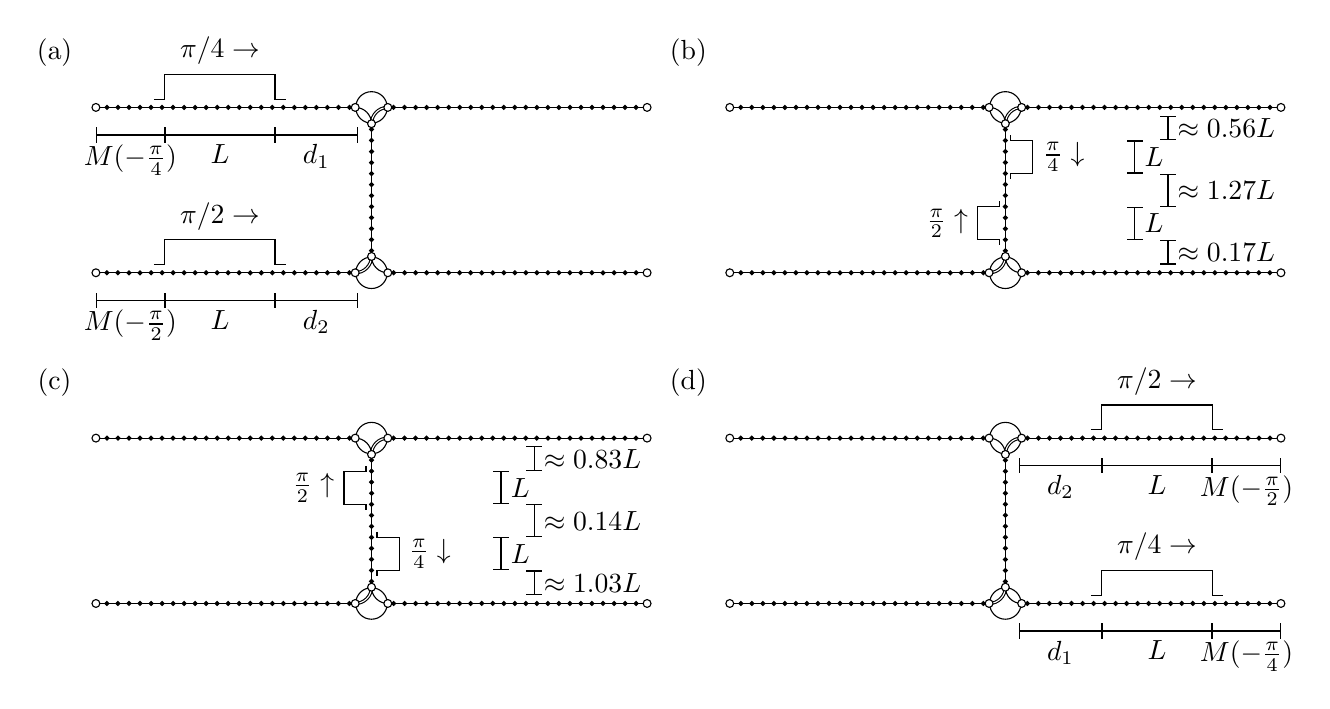
\begin{tikzpicture}[   scale=0.7,   
	dots/.style={circle,draw=black,fill=black,inner sep=0pt,minimum size=.5 mm}, 
	splitter/.style={circle,draw=black,fill=white,inner sep=0pt,minimum size=4mm},   
	attach/.style={circle,draw=black,fill=white,inner sep=0pt,minimum size=1mm}]
	
\begin{scope}[yshift= 6 cm]
  \node at (-.75,4) {(a)};

  \draw (0,0) to (10,0);   
  \draw (0,3) to (10,3);
  \foreach \x in {0,.2,.4,...,10}{
  \node at (\x, 0) [dots] {};
  \node at (\x, 3) [dots] {};
  }
  \foreach \y in {0,.2,.4,...,3}
  \node at (5,\y) [dots] {};
  
  \node (splitter42) at (5,0) [splitter] {};   
  \node (splitter41) at (5,3) [splitter] {};   
  \draw (splitter41.south) to (splitter42.north);      
  \draw (splitter41.west) to[out=0,in=90] (splitter41.south);   
  \draw[line width=1.2pt] (splitter41.south) to[out=90,in=180]           
  (splitter41.east);   
  \draw[line width=.4pt,white] (splitter41.south) to[out=90,in=180] (splitter41.east);
  \draw[line width=1.2pt] (splitter42.west) to[out=0,in=-90]           (splitter42.north);   
  \draw[line width=.4pt,white] (splitter42.west) to[out=0,in=-90]           (splitter42.north);   
  \draw (splitter42.north) to[out=-90,in=180] (splitter42.east);
  \node at (splitter41.east) [attach]{};
  \node at (splitter41.west) [attach]{};
  \node at (splitter41.south) [attach]{};
  \node at (splitter42.east) [attach]{};
  \node at (splitter42.west) [attach]{};
  \node at (splitter42.north) [attach]{};
  
  \node at (0,0) [attach]{};
  \node at (0,3) [attach]{};
  \node at (10,0) [attach]{};
  \node at (10,3) [attach]{};  

  \draw (1.05,3.15) to (1.25,3.15) to (1.25,3.6) to node[above]          
    {${\pi}/{4}\rightarrow$} (3.25,3.6) to (3.25,3.15) to (3.45,3.15);
  \draw (1.05,0.15) to (1.25,0.15) to (1.25,0.6) to node[above]          
    {${\pi}/{2}\rightarrow$} (3.25,0.6) to (3.25,0.15) to (3.45,0.15);
  \draw[|-|] (0,2.5) to node[below] {$M(-\frac{\pi}{4})$} (1.25,2.5);   
  \draw[|-|] (1.25,2.5) to node[below]{$L$}   (3.25,2.5);   
  \draw[|-|] (3.25,2.5) to node[below]{$d_1$} (4.75,2.5);
  \draw[|-|] (0,-.5) to node[below] {$M(-\frac{\pi}{2})$} (1.25,-.5);   
  \draw[|-|] (1.25,-.5) to node[below]{$L$}   (3.25,-.5);   
  \draw[|-|] (3.25,-.5) to node[below]{$d_2$} (4.75,-.5);
\end{scope}
  
%----------------------------------------------------------------------------------------%

\begin{scope}[xshift= 11.5cm, yshift=6cm]
  \node at (-.75,4) {(b)};

  \draw (0,0) to (10,0);   
  \draw (0,3) to (10,3);
  \foreach \x in {0,.2,.4,...,10}{
  \node at (\x, 0) [dots] {};
  \node at (\x, 3) [dots] {};
  }
  \foreach \y in {0,.2,.4,...,3}
  \node at (5,\y) [dots] {};
  
  \node (splitter42) at (5,0) [splitter] {};   
  \node (splitter41) at (5,3) [splitter] {};   
  \draw (splitter41.south) to (splitter42.north);      
  \draw (splitter41.west) to[out=0,in=90] (splitter41.south);   
  \draw[line width=1.2pt] (splitter41.south) to[out=90,in=180]           
  (splitter41.east);   
  \draw[line width=.4pt,white] (splitter41.south) to[out=90,in=180] (splitter41.east);
  \draw[line width=1.2pt] (splitter42.west) to[out=0,in=-90]           (splitter42.north);   
  \draw[line width=.4pt,white] (splitter42.west) to[out=0,in=-90]           (splitter42.north);   
  \draw (splitter42.north) to[out=-90,in=180] (splitter42.east);
  \node at (splitter41.east) [attach]{};
  \node at (splitter41.west) [attach]{};
  \node at (splitter41.south) [attach]{};
  \node at (splitter42.east) [attach]{};
  \node at (splitter42.west) [attach]{};
  \node at (splitter42.north) [attach]{};
  
  \node at (0,0) [attach]{};
  \node at (0,3) [attach]{};
  \node at (10,0) [attach]{};
  \node at (10,3) [attach]{};
  \begin{scope}[yshift = -10 cm]
    \draw (5.1,11.7) to (5.1,11.8) to (5.5,11.8) to node[right]          
      {$\frac{\pi}{4}\downarrow$} (5.5,12.4) to (5.1,12.4) to (5.1,12.5);
    \draw (4.9,11.3) to (4.9,11.2) to (4.5,11.2) to node[left]            
      {$\frac{\pi}{2}\uparrow$} (4.5,10.6) to (4.9,10.6) to (4.9,10.5);
    \draw[|-|] (7.95,12.85) to node[right] {$\approx 0.56L$} (7.95,12.4);   
    \draw[|-|] (7.35,12.4)  to node[right] {$L$}   (7.35,11.8);   
    \draw[|-|] (7.95,11.8)  to node[right] {$\approx 1.27L$} (7.95,11.2);   
    \draw[|-|] (7.35,11.2)  to node[right] {$L$}   (7.35,10.6);   
    \draw[|-|] (7.95,10.6)  to node[right] {$\approx 0.17L$} (7.95,10.15);
   \end{scope}  
\end{scope} 
  
%----------------------------------------------------------------------------------------%

  \node at (-.75,4) {(c)};

  \draw (0,0) to (10,0);   
  \draw (0,3) to (10,3);
  \foreach \x in {0,.2,.4,...,10}{
  \node at (\x, 0) [dots] {};
  \node at (\x, 3) [dots] {};
  }
  \foreach \y in {0,.2,.4,...,3}
  \node at (5,\y) [dots] {};
  
  \node (splitter42) at (5,0) [splitter] {};   
  \node (splitter41) at (5,3) [splitter] {};   
  \draw (splitter41.south) to (splitter42.north);      
  \draw (splitter41.west) to[out=0,in=90] (splitter41.south);   
  \draw[line width=1.2pt] (splitter41.south) to[out=90,in=180]           
  (splitter41.east);   
  \draw[line width=.4pt,white] (splitter41.south) to[out=90,in=180] (splitter41.east);
  \draw[line width=1.2pt] (splitter42.west) to[out=0,in=-90]           (splitter42.north);   
  \draw[line width=.4pt,white] (splitter42.west) to[out=0,in=-90]           (splitter42.north);   
  \draw (splitter42.north) to[out=-90,in=180] (splitter42.east);
  \node at (splitter41.east) [attach]{};
  \node at (splitter41.west) [attach]{};
  \node at (splitter41.south) [attach]{};
  \node at (splitter42.east) [attach]{};
  \node at (splitter42.west) [attach]{};
  \node at (splitter42.north) [attach]{};
 
  \node at (0,0) [attach]{};
  \node at (0,3) [attach]{};
  \node at (10,0) [attach]{};
  \node at (10,3) [attach]{};
  \begin{scope}[yshift = - 5cm]
  \draw (5.1,6.3) to (5.1,6.20) to (5.5,6.20) to node[right]            {$\frac{\pi}{4}\downarrow$} (5.5,5.6) to (5.1,5.6) to (5.1,5.5);
  \draw (4.9,6.7) to (4.9,6.8) to (4.5,6.8) to node[left]            {$\frac{\pi}{2}\uparrow$} (4.5,7.4) to (4.9,7.4) to (4.9,7.5);
  \draw[|-|] (7.95,7.85) to node[right] {$\approx 0.83L$} (7.95,7.4);   
  \draw[|-|] (7.35,7.4)  to node[right] {$L$}   (7.35,6.8);   
  \draw[|-|] (7.95,6.8)  to node[right] {$\approx 0.14L$} (7.95,6.2);   
  \draw[|-|] (7.35,6.2)  to node[right] {$L$}   (7.35,5.6);   
  \draw[|-|] (7.95,5.6)  to node[right] {$\approx 1.03L$} (7.95,5.15);
  \end{scope}
  
%----------------------------------------------------------------------------------------%
\begin{scope}[xshift=11.5cm]
  \node at (-.75,4) {(d)};

  \draw (0,0) to (10,0);   
  \draw (0,3) to (10,3);
  \foreach \x in {0,.2,.4,...,10}{
  \node at (\x, 0) [dots] {};
  \node at (\x, 3) [dots] {};
  }
  \foreach \y in {0,.2,.4,...,3}
  \node at (5,\y) [dots] {};
  
  \node (splitter42) at (5,0) [splitter] {};   
  \node (splitter41) at (5,3) [splitter] {};   
  \draw (splitter41.south) to (splitter42.north);      
  \draw (splitter41.west) to[out=0,in=90] (splitter41.south);   
  \draw[line width=1.2pt] (splitter41.south) to[out=90,in=180]           
  (splitter41.east);   
  \draw[line width=.4pt,white] (splitter41.south) to[out=90,in=180] (splitter41.east);
  \draw[line width=1.2pt] (splitter42.west) to[out=0,in=-90]           (splitter42.north);   
  \draw[line width=.4pt,white] (splitter42.west) to[out=0,in=-90]           (splitter42.north);   
  \draw (splitter42.north) to[out=-90,in=180] (splitter42.east);
  \node at (splitter41.east) [attach]{};
  \node at (splitter41.west) [attach]{};
  \node at (splitter41.south) [attach]{};
  \node at (splitter42.east) [attach]{};
  \node at (splitter42.west) [attach]{};
  \node at (splitter42.north) [attach]{};
 
  \node at (0,0) [attach]{};
  \node at (0,3) [attach]{};
  \node at (10,0) [attach]{};
  \node at (10,3) [attach]{};
  \draw (6.55,3.15) to (6.75,3.15) to (6.75,3.6) to node[above]            {${\pi}/{2}\rightarrow$} (8.75,3.6) to (8.75,3.15) to (8.95,3.15);
  \draw (6.55,.15) to (6.75,.15) to (6.75,.6) to node[above]            {${\pi}/{4}\rightarrow$} (8.75,.6)to (8.75,.15) to (8.95,.15);
  \begin{scope}[yshift=-.25cm]
  \draw[|-|] (5.25,2.75) to node[below] {$d_2$} (6.75,2.75);   
  \draw[|-|] (6.75,2.75) to node[below]{$L$}   (8.75,2.75);   
  \draw[|-|] (8.75,2.75) to node[below]{$M(-\frac{\pi}{2})$} (10,2.75);
  \draw[|-|] (5.25,-.25) to node[below] {$d_1$} (6.75,-.25);   
  \draw[|-|] (6.75,-.25) to node[below]{$L$}   (8.75,-.25);   
  \draw[|-|] (8.75,-.25) to node[below]{$M(-\frac{\pi}{4})$} (10,-.25);
  \end{scope}
\end{scope}
\end{tikzpicture} 
  \caption[$\CD$ gate cartoon]{This picture illustrates the scattering process for two wave-packets that are incident on the input paths as shown in figure (a) at time $t=0$. Figure (b) shows the location of the two wave-packets after a time $t_{1}$ and figure (c) shows the wave-packets after a time $t_{2}$. After the particles pass one another they acquire an overall phase of $e^{i\theta_\pm}$. Figure (d) shows the final configuration of the wave-packets after a total evolution time $t_{\CD}$.}
  \label{fig:11_scattering_cartoon}
\end{figure}


Additionally, note that the eigenstates of $H_G^2$ decompose into a symmetric and an antisymmetric subspace.  While it is intuitively more clean to work with distinguishable particles, the phases acquired during the evolution on $G$ will depend on the symmetry of the underlying particles.  As such, let us define the eight states
\begin{align}
  \ket{(z_1z_2)_{\text{in/out}}}_{\pm} &= \frac{1}{\sqrt{2} }\Big(\ket{(z_1)_{\text{in/out}}}^1 \ket{(z_{2})_{\text{in/out}}}^2 \pm \ket{(z_{2})_{\text{in/out}}}^2\ket{(z_1)_{\text{in/out}}}^1 \Big).
\end{align}
Our analysis will be for these states.

If we note that the input states don't particularly rely on the initial distance from the graph, and that the output states similarly don't rely on the distance from the end, we will be able to easily combine the time evolution on these graphs with the time evolution on other graphs.  Just so long as the initial wave-packets start a distance proportional to $L$ away from the ends, and similarly end a distance proportional to $L$ from the ends, we can us \lem{truncation} in order to determine the overall time evolution.

In particular, we have the following lemma:
\begin{lemma}
Let $G'$ be the graph given in \fig{explicit_cd} with distances given by \eq{Z_eq}--\eq{W_eq}, and where we assume that the initial and final states as defined in \eq{cd_input_1}, \eq{cd_input_2}, and \eq{cd_output_10}-\eq{cd_output_21} only have support on vertices a distance at least $L/3$ from the ends of the truncated paths.  If the momentum switch has transmission coefficient $T_1$ for momentum $k_1$ and transmission coefficient $T_2$ for momentum $k_2$, and if the phase acquired for two particle scattering between momentum $k_1$ and $k_2$ is given by $\theta_{\pm}$ for symmetric and antisymmetric states, then we have the following approximations for the time-evolved states:
\begin{align}
  \left\Vert e^{-iH_{G'}^{(2)}t_{\mathrm{II}}}|00_{\text{in}}\rangle_{\pm}-|00_{\text{out}}\rangle_{\pm} \right\Vert  & \leq \chi \sqrt{\frac{\log L}{L}}\label{eq:bound00}\\
  \left\Vert e^{-iH_{G'}^{(2)}t_{\mathrm{II}}}|01_{\text{in}}\rangle_{\pm}-T_{2}^2|01_{\text{out}}\rangle_{\pm}\right\Vert  & \leq \chi \sqrt{\frac{\log L}{L}}\label{eq:bound01}\\
  \left\Vert e^{-iH_{G'}^{(2)}t_{\mathrm{II}}}|10_{\text{in}}\rangle_{\pm}-T_1^2|10_{\text{out}}\rangle_{\pm}\right\Vert  & \leq\chi \sqrt{\frac{\log L}{L}}\label{eq:bound10}\\
  \left\Vert e^{-iH_{G'}^{(2)}t_{\mathrm{II}}}|11_{\text{in}}\rangle_{\pm} - e^{i\theta_{\pm}}T_1^2T_2^2|11_{\text{out}}\rangle_{\pm}\right\Vert  & \leq\chi \sqrt{\frac{\log L}{L}}.\label{eq:bound11}
\end{align}
\label{lem:cd_bounds}
\end{lemma}


\begin{proof}
The first three bounds \eq{bound00}, \eq{bound01}, and \eq{bound10} are similar to the proofs of \chap{SP_universality}, since in each case the two particles are supported on disconnected subgraphs and thus we can use \lem{disconnected_MPQW}.  For each of the single-particle scattering events, we can use a strategy similar to \lem{single_qubit_encoded_computation} to bound the error in our time-evolution for the unsymmetrized two-particle states.  To get the bound of \eq{bound11}, the proof strategy will be similar, but we will also need an application of \thm{two_particle_wave-packet_bound} during the times at which both particles are located on the long path.


Let us first understand the single-particle evolutions on the long paths. Note that $t_{\CD} \leq c L$ for some constant $c$, and thus according to \thm{single_particle_wavepacket_bound}, on an infinite path $P$ we have that
\begin{align}
  \bigg\Vert \gamma e^{- i P t } \sum_{\mu-L}^{\mu+L} e^{i k x} e^{-  \frac{(x-\mu)^2}{2\sigma} }\ket{x} - \gamma  e^{-2i t \cos(k)} \sum_{\mu(t) - L}^{\mu(t) + L} e^{ i k x} e^{- \frac{(x-\mu(t))^2}{2\sigma^2}} \ket{x} \bigg\Vert \leq \xi \sqrt{\frac{ \log L}{L}}
\end{align}
for some constant $\xi$ and where $\mu(t) = \mu + \lceil 2 t \sin(k)\rceil$.  While \thm{single_particle_wavepacket_bound} doesn't exactly give us this, if we apply the theorem to a graph gadget $\widehat{G}$ that results in the final graph being a long path, and assume that the initial location is far from the scattering event, the result follows after a relabeling of the basis states.  If we then note that the corresponding approximation involving $\mu(t)$ on the finite path always remains a distance at least $L/3$ away from the ends of the finite approximation, \lem{truncation} with $H = A(P)$, $\tilde{H} = A(G')$, and $N_0 = \frac{L}{3}$, and the error bound of $\delta =\xi \sqrt{\log L/L}$ gives us
\begin{align}
  \big\Vert e^{-i A(G') t_{\CD}} \ket{0_{\text{in}}}^i - \ket{0_\text{out}}^i\big\Vert &\leq \bigg( \frac{ 8 e t_{\CD}}{N_0} + 2 \bigg) \bigg[\xi \sqrt{\frac{\log L}{L}} + 2^{- N_0} \bigg( 1 - \xi \sqrt{\frac{\log L}{L}}\bigg)\bigg]\\
  & \leq \zeta \sqrt{ \frac{\log L}{L}}
\end{align}
for some constant $\chi$ that is independent of the momentum $k$.  Hence, we have that this approximation holds for both long paths.


Now let us analyze the single-particle evolution on the subgraph that connects the two particles.  For both particles, we will define approximations to the time-evolved wave-packets that will equal both the initial state and the corresponding final states.  Namely, if we also label the vertices of the path 5 (the one of length $Z$ which are currently labeled $(x,5)$) as $(W+1+x,2)$ and $(X + Z - x+2,3)$, then we can define the states 
\begin{align}
  \ket{\alpha_{1}^1(t)} &= \gamma e^{-2 i t \cos(k_1)} \sum_{x = \mu(t) - L}^{\mu(t) + L} e^{ i k_1 x} e^{-\frac{(x-\mu(t))^2}{2\sigma^2}} \ket{x,2}\\
  \ket{\alpha_{2}^1(t)} &= \gamma e^{-2 i t \cos(k_2)} \sum_{x = \nu(t) - L} ^{\nu(t) + L} e^{i k_2 x} e^{-\frac{(x-\nu(t))^2}{2\sigma^2}} \ket{x,3}
\end{align}
where $\mu(t) = \mu + \lceil 2 t \sin (k_1)\rceil$ and $\nu(t) = \nu + \lceil 2 t \sin (k_2)\rceil$.  Note that these are (almost) the same approximations as used for the long paths, where we assume that the momentum switches essentially act as connections between the correct long paths.

With these approximations, we will then want to show that the time evolution of the initial states approximately follow these output states, possibly with some additional phases.  In particular, note that there are three times (not including $t=0$) that are important for our evolution,
\begin{align}
  t_1 &= \frac{(4 +  \alpha)L}{2 \sin |k_1|}\\
  t_2 &= t_1 + \frac{6L}{\sin |k_1| + \sin |k_2|}\\
  t_{\CD} &= \frac{(11 +\alpha) L}{2 \sin |k_1|}.\label{eq:t_CD_defn}
\end{align}
If we can show that the time-evolved approximation at one time is close to the approximation at the next time for each of these times, we then have that our final approximation and the time-evolved initial state are close as well.  To do so, we will use the same procedure for combining our time-evolution on graphs as was done in \chap{SP_universality}.

Namely, we can use \lem{truncation} and \thm{single_particle_wavepacket_bound} to analyze the evolution of these states.  Note that \thm{single_particle_wavepacket_bound} gives us an approximation for the evolution of $\ket{\alpha^1_j(t)}$ via the momentum switch on the infinite path, and two applications of \lem{truncation} allows us to then analyze the evolution of the state for times $0 \leq t \leq t_1$ (after a suitable relabeling of the vertices).  In particular, we have that 
\begin{align}
  \Big\Vert e^{-i H_{G'}^{(1)} t_1 } \ket{\alpha_j^{1}(0)} - T_j \ket{\alpha_j^{1}(t_1)} \Big\Vert \leq \zeta_j^1\sqrt{\frac{\log L}{L}},
  \label{eq:two_particle_gadget_single_bound_1}
\end{align}
where the dependence of the constant on $j$ is only there in terms of the initial distance of the wave-packet from the ends of the finite paths.  


We can then use the same trick, namely two applications of \lem{truncation} and a single application of \thm{single_particle_wavepacket_bound} to understand the evolution on the path of length $Z$ between times $t_1$ and $t_2$.  Literally the same analysis as in the previous paragraph again gives us that
\begin{align}
  \Big\Vert e^{-i H_{G'}^{(1)} (t_2- t_1) } \ket{\alpha_j^{1}(t_1)} - \ket{\alpha_j^{1}(t_2)} \Big\Vert \leq \zeta_j^2\sqrt{\frac{\log L}{L}}
  \label{eq:two_particle_gadget_single_bound_2}
\end{align}
where again the constant only depends on the distance between the support of the approximation and the truncated ends, but in both cases is a constant.

Finally, a third application of this trick around the second momentum switch gives us
\begin{align}
   \Big\Vert e^{-i H_{G'}^{(1)} (t_{\CD}- t_2) } \ket{\alpha_j^{1}(t_2)} - T_j \ket{\alpha_j^{1}(t_\CD)} \Big\Vert \leq \zeta_j^3\sqrt{\frac{\log L}{L}},
     \label{eq:two_particle_gadget_single_bound_3}
\end{align}
where we again have used a necessary relabeling of the vertices.

Combining the three bounds \eq{two_particle_gadget_single_bound_1}--\eq{two_particle_gadget_single_bound_3}, we then have that
\begin{align}
  \Big\Vert e^{-i H_{G'}^{(1)} (t_{\CD}) } \ket{\alpha_j^{1}(0)} - T_j^2 \ket{\alpha_j^{1}(t_\CD)} \Big\Vert \leq (\zeta_j^1 + \zeta_j^2 + \zeta_j^3)\sqrt{\frac{\log L}{L}},
\end{align}
and thus we have approximations to the single-particle evolutions.

From this, if we use \lem{disconnected_MPQW} along with these three bounds on the evolution for times $t_{\CD}$, we have bounds similar \eq{bound00}, \eq{bound01}, and \eq{bound10} for the unsymmetrized states.  However, since the bounds (and approximations) don't depend on the symmetrization of the underlying states, we also have the symmetrized and antisymmetrized bounds as well.

Finally, we need to show the bound \eq{bound11}.  Unfortunately, this bound is slightly more difficult to prove, as we cannot naively use \lem{disconnected_MPQW}.  However, a more nuanced application of \lem{truncation} will allow us to approximate the evolution of both particles on $G'$ by the evolution on a disconnected graph for times less that $t_1$ and larger than $t_2$.  We will then only need to work with the two-particle interactions for times between $t_1$ and $t_2$, and here we will be able to use \lem{truncation} to approximate the analysis by that on an infinite path for both the symmetric and anti-symmetric states.  Putting everything together, we have a good approximations for all times $0 < t < t_{\CD}$, and thus we also have a good approximation for the final state.

To do this, let us define the graph $G^{\text{sep}}_1$ to be the $G'$ with the vertex labeled $(\lceil (3 + \alpha + 1/2)L\rceil, 5)$ removed and let $G^{\text{sep}}_2$ be $G'$ with the vertex labeled $(\lceil (3+1/2)L\rceil,5)$ removed.  Note that both $G^\text{sep}_i$ have four components, whereas $G'$ had three, but importantly that the two particles only have amplitude on separate components.  As such, we can then use \lem{disconnected_MPQW} and \lem{truncation} as in the case for any of the other logical computational basis states, at least for times in which the single-particle wave-packets remain far from the removed graph.  In particular, for all times $ 0 < t < t_1$, the approximation arising from the corresponding two-particle evolution on disconnected graphs (i.e., both the single-particle evolutions) remain a distance at least $L/3$ from the removed vertex.  Hence, using \lem{disconnected_MPQW} and the same single-particle evolutions as above, we have that
\begin{align}
  \Big\Vert e^{- i H_{G'}^{(2)} t_1} \ket{11_\text{in}} - T_1 T_2 \ket{\alpha_1^{1}(t_1)}\ket{\alpha_{1}^2 (t_1)} \Big\Vert \leq \xi_3 \sqrt{\frac{\log L}{L}}
\end{align}
for some constant $\xi_3$.  In particular, we have that each of the individual single-particle evolutions an the finite-sized graphs have errors bounded by $\xi_1$ and $\xi_2$ times $\sqrt{\log L/L}$ (as in the above examples), and thus the two-particle evolution on $G^{\text{sep}}$ has an error bound with constant $\xi_1 + \xi_2$.  Another application of \lem{truncation}, using the fact that we are dealing with two-particles and thus the norm of $H_{G'}^{(2)}$ is bounded, the approximations are far from the removed vertex, and our bound on the error when evolving on  $G^{\text{sep}}$, then gives the error as claimed.

At this point, our approximations to the time-evolved wave function are only supported on the long path far from the ends of the path, and thus we can use two applications of \lem{truncation} to look at the time-evolution on an infinite path.  This is exactly the reason for \thm{two_particle_wave-packet_bound}, and we can thus use it's bounds.  It is at this point that we discover different evolutions for symmetric and anti-symmetric particles, as the relevant phase acquired during the overlap is dependent on the symmetry between the particles.

In particular, if $P$ is the infinite path with vertices corresponding to the finite path of length $Z$, we have that \thm{two_particle_wave-packet_bound} gives us that
\begin{align}
  &\bigg \Vert e^{-i H_P^{2}(t_2-t_1)}\Big( \ket{\phi_{\lceil (2+\alpha)L\rceil}^{L,\sigma}(-k_1)}\ket{\phi_{\lceil (7+\alpha)L\rceil}^{L,\sigma}(k_2)} \pm  \ket{\phi_{\lceil (7+\alpha)L\rceil}^{L,\sigma}(k_2)}\ket{\phi_{\lceil (2+\alpha)L\rceil}^{L,\sigma}(-k_1)}\Big)\nonumber\\
  &\qquad - e^{i\theta_{\pm}}e^{-2i (t_2-t_2)(\cos k_1 + \cos k_2)} \Big( \ket{\phi_{4L}^{L,\sigma}(-k_1)}\ket{\phi_{2L}^{L,\sigma}(k_2)} \pm  \ket{\phi_{2L}^{L,\sigma}(k_2)}\ket{\phi_{4L}^{L,\sigma}(-k_1)}\Big)\bigg\Vert\nonumber\\
  &\qquad\qquad \leq \xi_4 \sqrt{\frac{L}{L}},
\end{align}
with an approximation for all intermediate times that has a similar bound.  With two applications of \lem{truncation}, along with a relabelling of vertices, we can see
\begin{align}
  \Big \Vert e^{-i H_G'^{(2)} (t_2 - t_{1})}\ket{\alpha_1^1(t_1),\alpha_2^1(t_1)}_{\pm} - e^{i\theta_{\pm}}\ket{\alpha_1^1(t_2),\alpha_2^1(t_2)}_{\pm} \Big \Vert  \leq \zeta_4 \sqrt{\frac{\log L}{L}}.
\end{align}


After the two particles have moved passed each other and we have reach time $t_2$, we can use the same trick to approximate the time evolution for $t_2 < t < t_{\CD}$ as for the early times, except on the graph $G_2^{\text{sep}}$.  We find that the error in our approximation for these times is bounded by the same value as for the early times, as the analysis is nearly identical.  

If we then put together these three bounds, we have:
\begin{align}
  &\Big\Vert e^{- i H_G'^{(2)} t_{\CD}} \ket{11_{\text{in}}}^{1,2}_{\pm} - e^{i\theta_{\pm}} T_1^2 T_2^2 \ket{11_{\text{out}}}_{\pm}^{1,2}\Big\Vert\\
  & \qquad \leq \Big \Vert e^{-i H_G'^{(2)} t_{1}} \ket{\alpha_1^1(0),\alpha_2^1(0)}_{\pm}  - T_1T_2\ket{\alpha_1^1(t_1),\alpha_2^1(t_1)}_{\pm} \Big \Vert \nonumber\\
  &\qquad\qquad
  + \Big \Vert e^{-i H_G'^{(2)} (t_2 - t_{1})}\ket{\alpha_1^1(t_1),\alpha_2^1(t_1)}_{\pm} - e^{i\theta_{\pm}}\ket{\alpha_1^1(t_2),\alpha_2^1(t_2)}_{\pm} \Big \Vert \nonumber\\
  &\qquad\qquad
  + \Big \Vert e^{-i H_G'^{(2)} (t_{\CD}-t_{2})}\ket{\alpha_1^1(t_2),\alpha_2^1(t_2)}_{\pm} - T_1T_2\ket{\alpha_1^1(t_\CD),\alpha_2^1(t_\CD)}_{\pm} \Big \Vert\\
  & \qquad \leq\xi_5 \sqrt{\frac{\log L}{L}}
\end{align}
and we have \eq{bound11}.

If we then take $\chi$ to be the maximum constant for our four bounds, we have proven the theorem.
\end{proof}

At this point, we now understand how our assumed initial state propagates for single- and two-particle states, and we have the necessary building blocks for our universality result.  

Note that if $\theta_{+}(k_1,k_2) = \theta_{-}(k_1,k_2)$, then our results from above hold for distinguishable particles as well, since the applied unitary is then the same for all linear combinations of the two states.

\subsection{$n$-qubit evolution}

With our analysis of \lem{cd_bounds}, we can apply an encoded $\CD$-gate between two qubits, assuming the appropriate gadgets exist.  However, we are actually interested in the $n$-particle evolution, and before we turn our attention to combining several gates we need to extend our analysis to the case of $n$-qubits.

This will actually be very similar to that of \lem{MP_u_single_qubit_encoded_computation}, in that we will assume that our encoded initial state has each particle on separate components of a graph, except for the two particles on the graph $G$ that will be used to implement the encoded $\CD$-gate.  In particular,  let $G'$ be the infinite graph with $2(n-2)$ infinite paths, and the infinite version of \fig{explicit_cd} (i.e., $X = W = \infty$).  Assuming that we want to apply the encoded $\CD$ gate between qubits $j_1$ and $j_2$, and that we want the wave packet for qubit $\ell$ to be centered a distance $\mu_\ell$ from the first edge of the path, we then let $G(\vec{K})$ be the finite restriction of $G$.  In particular, we have that for the two qubits we want to interact, we have a copy of \fig{explicit_cd} where \eq{Z_eq}--\eq{W_eq} define the lengths, and for each qubit not involved in the applied unitary, there are two paths of length $2\mu_\ell + \lceil 2 t_{\CD} \sin |k_\ell |\rceil$.  We then have that the labelling scheme for the vertices in the copy of \fig{explicit_cd} are as in the previous section, while the remaining vertices are labelled as $(\ell,z,x)$ for $\ell\in [n]$ with $\ell\neq j_1,j_2$, $x\in [2\mu_\ell + \lceil 2 t_{\CD} \sin |k_\ell |\rceil]$ and $z\in \FF_2$.

With this labelling scheme for the vertices, we have that our initial logical states for qubits not affected by the unitary are given by
\begin{align}
  \ket{z}_{\text{log},\text{in},\ell} = \gamma \sum_{x = -\mu_\ell-L}^{-\mu_\ell + L} e^{- i k_\ell x} e^{ - \frac{(x-\mu_\ell)^2}{2\sigma^2}} \ket{\ell,x,z},
\end{align}
(exactly as in \lem{MP_u_single_qubit_encoded_computation}) with output encoded states given by
\begin{align}
  \ket{z}_{\text{log},\text{out},\ell} = \gamma e^{-2i T \cos(k_\ell)} \sum_{x = \mu_\ell-L}^{\mu_\ell + L} e^{- i k_\ell x} e^{ - \frac{(x-\mu_\ell)^2}{2\sigma^2}} \ket{\ell,x,z+1}.
\end{align}
For the two qubits affected by the $\CD$-gate, we have that the input encoded logical states are given by \eq{cd_input_1} and \eq{cd_input_2}, while the encoded logical output is given by \eq{cd_output_10}--\eq{cd_output_21}.  We then have that the $n$-qubit state $\ket{\phi} = \sum_{x\in \FF_2^n} \alpha_x\ket{x}$ is represented by
\begin{align}
  \ket{\phi}_{\text{log,in}} = \sum_{x\in \FF_2^n} \alpha_{x} \bigotimes_{i=1}^n \ket{x_i}_{\text{log},\text{in,i}}\label{eq:MP_two_input_encoding}
\end{align}
and for a given unitary $U$,
\begin{align}
  \ket{U\phi}_{\text{log,out}} = \sum_{x,y\in \FF_2^n} U_{xy}\alpha_{y} \bigotimes_{i=1}^n \ket{x_i}_{\text{log},\text{in,i}}.\label{eq:MP_two_output_encoding}
\end{align}

Note that these logical encodings assume that the $i$-th particle is used to represent the $i$-th qubit.  The fact that these particles are distinguishable will make our theorem difficult, so we will work with the states
\begin{align}
  \ket{\phi}_{\text{log,in/out}}^{\pm} = \frac{1}{\sqrt{2}} \big(\ket{\phi_{\text{log,in/out}}} \pm V_{(j_1j_2)} \ket{\phi_{\text{log,in/out}}}\big). 
\end{align}
Note that these states are symmetric (antisymmetric) between the two particles that interact, which will be sufficient for our purposes.  Further, since the Hamiltonian $H_{G}^N$ is permutation invariant, we will have the same result for any $V_\pi \ket{\phi}_{\text{log,in/out}}$.


We then have the following theorem on the evolution of a given logical state.

\begin{lemma}
\label{lem:MP_u_two_qubit_encoded_computation}
  Let $k_j\in (-\pi,0)$ for all $j\in [n]$, and let us assume that there exists a momentum switch between $k_{j_1}$ and $k_{j_2}$.  Let the logical states $\ket{z}^{\pm}_{\text{log},\text{in}}$ and $\ket{z}^{\pm}_{\text{log},\text{out}}$ be defined as in \eq{MP_single_input_encoding} and \eq{MP_single_output_encoding}, and let $G(\vec{K})$ be defined as above, where each $\mu_\ell \geq (1+\beta) L $.  We then have that there exists some constant $\xi$ such that for all $0 \leq t \leq t_{\CD}$ and any interaction $\mathcal{U}$,
\begin{align}
  \Big\Vert e^{-i H_G^N t} \ket{\phi(0)}^{\pm} - \ket{\phi(t)}^{\pm} \Big\Vert \leq \xi n \sqrt{\frac{\log L}{L}},
\end{align}
where
\begin{align}
  \ket{\phi(t)}^{\pm} = \sum_{x\in\FF_2^n} \alpha_x W_\pi \Bigg[\ket{\beta_{x_{j_1}x_{j_2}}(t)}^{\pm}\otimes\bigotimes_{\substack{\ell=1\\\ell\neq j_1,j_2}}^n   \ket{\alpha^{x_\ell}_\ell(t)}\Bigg],
\end{align}
the $\ket{\beta_{x_{j_1}x_{j_2}}(t)}$ are the approximations used in \lem{cd_bounds} for the logical input $x_{j_1}x_{j_2}$, $W_\pi$ is the permutation that takes the $j_1$-st particle to the first location, the $j_2$-nd particle to the second equation, and orders the rest of the particles,  and 
\begin{align}
  \ket{\alpha_\ell^z(t)} = \gamma e^{-2it \cos (k_\ell)} \sum_{x = \mu_\ell(t)-L}^{\mu_\ell(t) + L} e^{- i k_\ell x} e^{ - \frac{(x-\mu_\ell(t))^2}{2\sigma^2}} \ket{\ell,x,z},
\end{align}
with
\begin{align}
  \mu_\ell(t) &= \mu_\ell + 2t \sin |k_\ell|.
\end{align}
In particular, we have
\begin{align}
  \Big\Vert e^{-i H_G^N T} \ket{\psi}_{\text{log},\text{in}}^{\pm} - \ket{U\psi}_{\text{log},\text{out}}^{\pm} \Big\Vert \leq \xi n\sqrt{\frac{\log L}{L}}.
\end{align}
where $U$ is a diagonal two-qubit unitary given by $\diag\{1,T_2^2,T_1^2,T_1^2T_2^2e^{i\theta_\pm}\}$, where $T_j$ is the transmission coefficient for the momentum switch at momentum $k_j$, and $\theta_\pm$ is as in \lem{cd_bounds}.
\end{lemma}

\begin{proof}
  The proof of this theorem follows nearly identically to that of \lem{MP_u_single_qubit_encoded_computation}, in that we use \lem{disconnected_MPQW} to break the analysis into the components of the graph, and then use our results on each component.

Using the fact that the states $\ket{\phi(t)}$ all have the particles supported on different components of $G$ (except for $j_1$ and $j_2$), we have  by \lem{disconnected_MPQW} that
  \begin{align}
    e^{-i H_G^N t} \ket{\phi(0)}^\pm &= \big( e^{-i H_G'^2 t)}\big)^{(j_1,j_2)}\prod_{\substack{\ell=1\\\ell\neq j_1j_2}}^n \big( e^{-i A(G_\ell)t}\big)^{(\ell)} \ket{\phi(0)},
  \end{align}
where $G_\ell$ is the component on which the $\ell$-th particle is located.  However, we have that each of these unitaries commute, and
  \begin{align}
    \big( e^{-i A(G_\ell)t}\big)^{(\ell)} \ket{\phi(0)}&= \sum_{x\in \FF_2^n} \alpha_x \bigotimes_{i=1}^n e^{- i \delta_{i,\ell} A(G_\ell) t} \ket{\alpha_i^{x_i}(0)}\\
    & = \sum_{x\in \FF_2^n} \alpha_x \Bigg[\bigotimes_{i=1}^n \Big(\ket{\alpha_i^{x_i}(\delta_{\ell,i} t)} + \delta_{\ell,i} \ket{\epsilon_{\alpha_x,\ell}(t)}\Big)\Bigg],
  \end{align}
  by \lem{single_qubit_encoded_computation}, with $\Vert \ket{\epsilon_{\alpha_x,\ell}(t)}\Vert \leq \xi \sqrt{\log L/L}$ for some constant $\xi$.  
  
  Additionally, we have from \lem{cd_bounds} that
  \begin{align}
    e^{-i H_{G'}^2 t }\ket{\beta_{x_{j_1}x_{j_2}}(0)} &= \ket{\beta_{x_{j_1}x_{j_2}}(t)} + \ket{\xi_{x_{j_1},x_{j_2}}(t)},
  \end{align}
  where $\Vert  \ket{\xi_{x_{j_1},x_{j_2}}(t)}\Vert \leq \xi\sqrt{\log L/L}$
  
  
  Combining these results, we then have that
  \begin{align}
    e^{-i H_G^N t} \ket{\phi(0)} &= \sum_{x\in \FF_2^n} \alpha_x \Bigg[\bigotimes_{i=1}^n \Big(\ket{\alpha_i^{x_i}(t)} + \ket{\epsilon_{\alpha_x,\ell}(t)}\Big)\Bigg]\\
      &= \ket{\phi(t)} + \ket{\varepsilon(t)},
  \end{align}
  where $\Vert \ket{\varepsilon(t)}\Vert \leq n \xi \sqrt{\log L/L}$.
\end{proof}

From this, we then have the relevant bounds on the multi-qubit evolution.

%\subsection{Explicit momenta}
%
%Show that BH with momenta $\pi/2$ and $\pi/4$ with interaction strength $\sqrt{2} + 2$

%%%%%%%%%%%%%%%%%%%%%%%%%%%%%%%%%%%%%%%%%%%%%%%%%%%%%%%%%%%%%%%%%%%%%%%%%%
%  Multi-gate simulation
%

\section{Multi-gate simulation}\label{sec:MP_multi_gate_simulation}

At this point, we know how to encode $n$ qubits into the MPQW of $n$-particles, we can simulate a single-qubit unitary on one of the qubits, assuming an appropriate gadget exists, and we can perform an entangling gate between two qubits, assuming the existence of a particular momentum switch and nontrivial phase in the two-particle scattering.  As such, if we can show how to combine these results without a large increase in the error, we will have our universality result.

Note that there are several arbitrary choices in this construction, as a proof of universality only requires the existence of a simulating graph; we expect that other choices would also provide universal simulation.  Additionally, our choice depends on the particular interaction Hamiltonian used in the MPQW, as the phase of the entangling gate $\CD$ depends on the interaction between the particles.  

Along those lines, let us fix some interaction $\mathcal{U}$ between the particles, and let us assume that $\Vert H_{\text{int}}^n \Vert \leq \gamma n^\nu$, for some constant $\gamma$ and $\nu$.  We will show almost all such interactions can be used for universal quantum computation.

We will assume that we want to simulate a circuit $\mathcal{C}_X = U_mU_{m_1}\cdots U_1$, where each $U_i$ is from some finite gate set.  After making our choices for our encoding, we will place some restrictions on this gate set related to the existence of certain scattering gadgets and the phase $\theta_{\pm}$ for two-particle interactions arising from $H_{\text{int}}$.

\subsection{Encoded qubits}

The first step in our construction will be to choose how to encode our qubits.  As in \sec{MP_qubit_encoding}, we will encode each qubit via a particle in a dual-rail encoding, where the logical states are given by \eq{MP_u_logical states}.  At this point, however, we need only choose the values of $k_i$ for each qubit and the initial location of the center of the particles, $\mu_i$.

From our results in \sec{entangling_gate}, our construction will require at least two different momenta in order to simulate an entangling gate.  We will make the choice to only use two momenta, $k_1$ and $k_2$, where $\sin |k_1| \leq \sin |k_2|$ and where there exists a momentum switch between the two particles.  We also assume that for $k_1$ and $k_2$, there are scattering gadgets that implement a universal set of single-qubit unitaries.  Note that several such pairs of momentum are known from \chap{scattering_gadgets}. 

Additionally, for our most simple scheme, we will assume that the particles indistinguishable.  All of our results from this chapter will hold with this assumption, and in addition we will easily be able to use \lem{MP_u_two_qubit_encoded_computation}.  Assuming that $\theta_{+}(k_1,k_2) \neq 0$, we will assume that our particles are bosons, but if $\theta_{+}(k_1,k_2) =0$ we will assume the particles are fermions.  If both $\theta_{\pm}(k_1,k_2) = 0$, note that our entangling gate cannot be constructed at this pair of momenta.

With these choices, we will choose for the $n$-th qubit to have momentum $k_2$, while the remaining $n-1$ qubits will have momentum $k_1$.  With this choice, we will require that all two-qubit gates affect the $n$-th qubit, and thus it will act as a mediator qubit.  Further, we assume that each Gaussian wave-packet has a cut-off length $L$, with standard deviation $\sigma = \frac{L}{2\sqrt{\log L}}$.

\subsection{Constructing the simulating graph}

At this point, we have chosen our logical states, and we now want to construct the graph for our simulation.  Note that the idea behind this is almost the same as in \chap{SP_universality}, in that we build the simulating graph by concatenating scattering events.  In particular, for each unitary $U_i$, we will include a single-gate circuit of the form described in \sec{MP_single_qubit_gate_simulation} or \sec{entangling_gate}.  We then combine these graphs by removing the output paths from the graph  $U_{i}$, and connecting the corresponding trailing edges to the input paths of $U_{i+1}$.  An example of such combinations is given in \fig{combining_graphs}.

More concretely, for single-qubit unitary $U_i$, we will include a graph of the form described in \sec{MP_single_qubit_gate_simulation} with the scattering event corresponding to the unitary $U_i$ on the correct qubit.  We will assume that each $K_j$ for $j<n$ is equal to $4L-1$, and that 
\begin{align}
  K_n = \bigg\lceil 4 L \frac{ \sin |k_2|}{\sin |k_1|}\bigg\rceil - 1.
\end{align}
The reason for these choices is that we want a particle (with momentum $k_1$) to travel from a position centered at $-2L$ to a position centered about $2L$ during each single-qubit gate, and $K_n+1$ is the corresponding distance a particle with momentum $k_2$ travels.  Further, we want that the this centered position to be equidistant from the endpoints of the long paths and the corresponding locations where the graph gadgets are attached.  In this way, if we combine multiple scattering events implement a single-qubit unitary to the same qubit, when the wave-packet is centered it is a distance $2L-1$ from both gadgets.

Additionally, for each two-qubit unitary $U_i$, we will include a graph of the form described in \sec{entangling_gate}, with the choice of $M(k_1) = 2L-1$ and $M(k_2) = \lceil 2 L\sin |k_2|/\sin |k_1|\rceil -1$.  This choice of $M(k_i)$ is done to facilitate the attachment between graphs at neighboring times.

To combing the graphs for the unitaries $U_i$, for each $i < m$, we remove the rightmost $2L-1$ vertices from each outgoing path from $U_i$, and remove the leftmost vertex from each input path for $U_{i+1}$.  For each qubit $j\in [n]$ and each logical state $z\in \FF_2$, we then add an additional edge from the rightmost outgoing vertex from the modified graph for $U_i$ on the path corresponding to logical $z_j$ to the corresponding leftmost vertex of the modified graph of $U_{i+1}$. 

We can think of this in another manner, in that instead of removing the vertices, we simply identify the vertex $(i,x,j,z)$ (where $i$ identifies which unitary the vertex belongs to) with the vertex $(i+1,x-4L,j,z)$ if $j\neq n$ (where we assume that the unitary $U_i$ and $U_{i+1}$ are both single-qubit unitaries that do not affect qubit $j$).  We have a similar results for $j=n$, except that $(i,x,n,z)$ is identified with $(i+1,1- 2M(k_2) + x,z)$.  In the case where $U_i$ is a two-qubit unitary, we have a similar result.

Let the resulting graph be called $G_{X}$

\begin{figure}
  \centering
  \tikzsetnextfilename{MP_combining_graphs}
  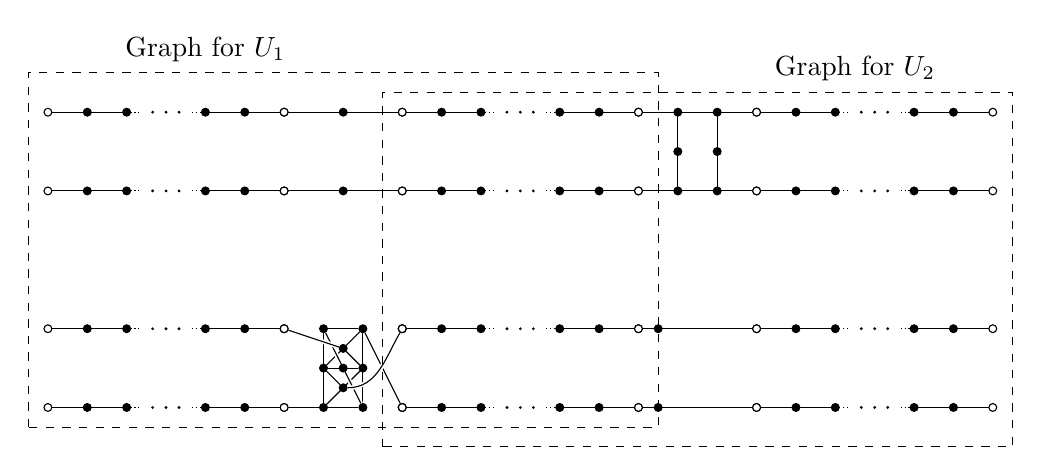
\begin{tikzpicture}[scale=.5,
  attach/.style={circle,fill=white,draw=black,
    inner sep=1pt,minimum size=0pt},
  vert/.style={circle,draw=black,fill=black,
    inner sep=1pt,minimum size=0pt},
  dots/.style={circle,fill=black,inner sep=.4pt,
    minimum size=0pt}
  ]
  \foreach \xsh in {0,9,18}{
  \foreach \ysh in {0,2,5.5,7.5}{
  \begin{scope}[xshift=\xsh cm,yshift=\ysh cm]
    \draw (0,0) -- (2,0);
    \draw (4,0) -- (6,0);
    \draw[densely dotted] (2,0) -- (2.33,0);
    \draw[densely dotted] (3.66,0) -- (4,0);

    \node at (0,0) [attach] {};
    \node at (1,0) [vert]{};
    \node at (2,0) [vert]{};
    \node at (2.66,0) [dots]{};
    \node at (3,0) [dots]{};
    \node at (3.33,0) [dots]{};
    \node at (4,0) [vert]{};
    \node at (5,0) [vert]{};
    \node at (6,0) [attach]{};
  \end{scope}}}



  \begin{scope}[xshift=6cm]
    \node (0inhad) at (0,2) [attach]{};
    \node (1inhad) at (0,0) [attach]{};
    \node (0outhad) at (3,2) [attach]{};
    \node (1outhad) at (3,0) [attach]{};
    
    \node (1had) at (1,0) [vert]{};
    \node (2had) at (2,0) [vert]{};
    \node (3had) at (1.5,.5) [vert]{};
    \node (4had) at (1,1) [vert]{};
    \node (5had) at (1.5,1) [vert] {};
    \node (6had) at (2,1) [vert] {};
    \node (7had) at (1.5,1.5) [vert]{};
    \node (8had) at (1,2) [vert]{};
    \node (9had) at (2,2) [vert]{};

    \draw (8had) -- (1had);
    \draw (9had) -- (2had);
    \draw (4had) -- (9had);
    \draw (1had) -- (6had);
    \draw (4had) -- (6had);
    \draw (3had) -- (4had);
    \draw (7had) -- (6had);
    \draw (1inhad) -- (2had);
    \draw (8had) -- (9had);
    \draw (8had) -- (5had)[ultra thick,white];
    \draw (5had) -- (2had)[ultra thick,white];
    \draw (8had) -- (2had);
    
    \draw (9had) -- (1outhad);
    \draw (0inhad) -- (7had)[ultra thick,white];
    \draw (0inhad) -- (7had);

    \draw (3had) to[out=0,in=240] (0outhad)[ultra thick,white];
    \draw (3had) to[out=0,in=240] (0outhad);

    \node at (0inhad) [attach]{};
    \node at (1outhad) [attach]{};
    \node at (0outhad) [attach]{};

  \end{scope}



  \draw (15,0) -- (18,0);
  \draw (15,2) -- (18,2);
  
  \node at (15,0) [attach] {};
  \node at (18,0) [attach] {};
  \node at (15,2) [attach] {};
  \node at (18,2) [attach] {};



  \begin{scope}[xshift=6cm,yshift = 5.5cm]
    \draw (0,0) -- (3,0);
    \draw (0,2) -- (3,2);
%    \draw[xshift=.5cm] (1,0) -- (1,.59) -- (.58,1) --  (1,1.42) 
%       -- (1.42,1) -- (1,.59);

    \node at (0,0) [attach]{};
    \node at (1.5,0) [vert] {};
    \node at (3,0) [attach]{};
%    \node at (1.5,.59) [vert]{};
%    \node at (1.08,1) [vert]{};
%    \node at (1.92,1) [vert]{};
 %   \node at (1.5,1.42) [vert]{};
  %  \node at (1,2) [vert]{};
 %   \node at (2,2) [vert]{};
    \node at (1.5,2) [vert]{};
    \node at (0,2) [attach]{};
    \node at (3,2) [attach]{};
  \end{scope}



  \begin{scope}[xshift=15cm,yshift=5.5cm]
    \draw (0,0) -- (3,0);
    \draw (0,2) -- (3,2);
    \draw (1,0) -- (1,2);
    \draw (2,0) -- (2,2);

    \foreach \x in {1,2}{
    \foreach \y in {0,1,2}{
      \node at (\x,\y) [vert]{};
    }}

    \foreach \x in {0,3}{
    \foreach \y in {0,2}{
      \node at (\x,\y) [attach]{};
    }}

  \end{scope}

\node at (15.5,2) [vert]{};
\node at (15.5,0) [vert]{};

%  \foreach \x in {0,9,18}{
%  \draw[xshift=\x cm,yshift=2.4cm,|-|] (-.25,0) 
%&      to node[above]{$L+2M(-\pi/2)$} (6.25,0);
  
%  \draw[xshift=\x cm,yshift=5.1cm,|-|] (-.25,0)
%      to node[below]{$L+2M(-\pi/4)$} (6.25,0);
%  }    

  \draw [dashed] (-.5,-.5) rectangle (15.5,8.5);

  \draw [dashed] (8.5,-1) rectangle (24.5,8);

  \node at (4,9.1) {Graph for $U_1$};

  \node at (20.5,8.6) {Graph for $U_2$};

\end{tikzpicture} 
  \caption[Combining graph example]{An example of concatenating two single-gate graphs.  The particular gadgets are between momenta $k_1 = -\frac{\pi}{4}$ and $k_2 = -\frac{\pi}{2}$.}
  \label{fig:combining_graphs}
\end{figure}

\subsection{Evolution analysis}

Now that we have our defined graph, we will want to show that the $n$-particle quantum walk on $G_X$ simulates the circuit $\mathcal{C}_X$.  We will do this by repeated application of the truncation lemma, so that we can analyze the evolution of the state iteratively.  In particular, if the particle is moving toward the graph gadget for the $i$-th unitary (and is sufficiently far from the graph gadget implementing the $(i-1)$-st unitary), we can use the truncation lemma to approximate the analysis using our results on the scattering behavior for the $i$-th graph (and only the $i$-th graph).  After the particles have proceeded with the appropriate scattering events and are leaving the $i$-th graph, we then repeat the process.  If we can show that each such gate implements a logical $U_i$ on the encoded space without leaving much error, we will have that the simulation is a success.

Along these lines, we will need to define encoded logical states for both input and output, as well as the logical states between unitaries.  If we let 
\begin{align}
  t_{\text{single}} = \frac{2L}{\sin |k_1|},
\end{align}
and remember the definition for $t_{\CD}$ in \eq{t_CD_defn}, we have that these are the two times required to implement a single-qubit gate ($t_{\text{single}}$) and to implement a two-qubit gate ($t_{\CD}$).  Additionally, let us define $m+1$ times, where $t_0 = 0$ and 
\begin{align}
  t_{i+1} = \begin{cases} t_i + t_{\text{single}} & U_i \text{ is a single-qubit gate}\\
    t_i + t_{\CD} & U \text{ is a two-qubit gate}.\end{cases}
\end{align}
In this manner, each time $t_i$ is after the $i$-th scattering event and before the $i+1$-th scattering event.  We will also have that at these times, the wave-packets for each qubit should be centered between scattering events.  

Let us now define our logical input and output states for each qubit at time $t_i$.  The most simple case is given at $t=0$, as the input logical states are exactly the symmetrized states from \eq{MP_single_input_encoding} if the first unitary is a single-qubit gate or the symmetrized states \eq{MP_two_input_encoding} if the first unitary is a two-qubit unitary (additionally, let us label this basis by $1$, since it correspond to the first logical basis).  Assuming that the initial state is the logical 0 state, we then have that at time $t_1$, the state is of the form
\begin{align}
  e^{-i H_{G_X}^N t_1} \ket{0}_{\text{log,in},1}.
\end{align}
If we then use \lem{truncation} for the vertices of the graph $G_X$ that arose from the graph implementing $U_1$, along with our approximation to the evolution according to $G_1$ given by either \lem{MP_u_single_qubit_encoded_computation} or \lem{MP_u_two_qubit_encoded_computation}, we can see that for all times $0\leq t \leq t_1$, the support of our approximation to evolution according to the truncated Hamiltonian remains a distance $\frac{L}{2}$ from the removed vertices.  Using the error bounds from the appropriate lemma, we then have that 
\begin{align}
  e^{-iH_{G_X}^N t_1} \ket{0}_{\text{log,in},1} = \ket{U_1 0}_{\text{log,out},1} + \ket{\epsilon}
\end{align}
where 
\begin{align}
  \big \Vert \ket{\epsilon} \big\Vert \leq \xi n \Vert H_{G_X}^n \Vert \sqrt{\frac{\log L}{L}}, \label{eq:single_gate_error}
\end{align}
for some constant $\xi$.

Additionally, note that the output logical states for the first unitary have the exact form as the input logical states to the second unitary (by construction), except for a global phase resulting from a change of vertex labelling between the two graphs computing the unitaries and the acquired phase from the energy.  As such, we repeat the above process with the truncation lemma to evolve $\ket{U_1 0}_{\text{log,out},1}$ according to $G_2$ for times $t_1 \leq t \leq t_2$, while only acquiring an additional error of \eq{single_gate_error}.  

We can repeat this process for each unitary $U_i$, until we get that 
\begin{align}
  \bigg\Vert e^{-i H_{G_X}^N t_1} \ket{0}_{\text{log,in},1} - e^{i\phi} \ket{U_m U_{m-1}\cdots U_1 0}_{\text{log,out},m} \bigg\Vert \leq \xi m n \Vert H_{G_X}^n \Vert \sqrt{\frac{\log L}{L}},
\end{align}
where $\phi$ is a global phase that doesn't affect the logical state.  

From this, if we then choose 
\begin{align}
  L = \Theta\Big( m^2 n^2 \Vert H_{G_X}^n \Vert^2 \log(m n)\Big),
\end{align}
we can make the error in the evolution constant. (Note that we used our bound on $\Vert H_(G_X)^n\Vert$ in the logarithm.)  From this, we then have that the total number of vertices of our graph will be $\OO(m^3 n^3 \Vert H_{G_X}^n \Vert^2 \log(m n))$ and the total evolution time will be $\OO(m^3 n^2 \Vert H_{G_X}^n \Vert^2 \log(m n))$.  In the case of the Bose-Hubbard model and the most simple nearest-neighbor interactions, we have that $\Vert H_{G_X}^n\Vert \leq \gamma n^2$, and these bounds become $\OO( m^3 n^7 \log(mn))$ and $\OO(m^3 n^6 \log(mn))$.

I would like to point out that this is a near quadratic improvement over the results of Childs, Gosset, and Webb \cite{MPQW}.  This occurred by the novel analysis using Gaussian states.

\subsection{Universality}

At this point, we have only shown how to simulate a circuit of a particular form.  Namely, our construction requires that each unitary $U$ in the circuit comes from a gate set where 
\begin{align}
  U \in \begin{cases}
    S_{k_2} & \text{ if $U$ is a single-qubit gate and acts on qubit $n$}\\
    S_{k_1} & \text{ if $U$ is a single-qubit gate otherwise}\\
    \CD_{i,n} & \text{otherwise},
  \end{cases}
\end{align}
and where $S_{k_i}$ requires the existence of a particular scattering gadget and $\CD_{i,j}$ is a single gate.  However, if we assume that each $S_{k_i}$ is a universal set of single-qubit gates, and if we assume that the phase acquired between $k_1$ and $k_2$ when they interact on a long path is $\alpha \pi$, for some irrational $\alpha$, then we can approximate a $\CNOT_{i,n}$ gate and a $\CNOT_{n,i}$ gate.  We can then use these $\CNOT$ gates to implement swap gates, and thus we have approximate $\CNOT_{i,j}$ gates between all pairs of qubits.  Combining this with the universal single-qubit gate set for all qubits, we then have that we can approximate an arbitrary circuit with circuits of the form required for our construction.

Note that the acquired phase is a ration function of $e^{ik_1}$, $e^{i k_2}$, and the interaction strength, and thus for almost all values of the interaction strength we have that the acquired phase is an irrational multiple of $\pi$.  From this, we have that MPQW with almost any interaction is universal for quantum computing.

\subsubsection{$k_1 = -\frac{\pi}{4}$ and $k_2 = -\frac{\pi}{2}$}

Note from \sec{gadgets_unitary}, we have a universal gate set for both $k_1$ and $k_2$.  Further, we have from \chap{MPQW} that for onsite interactions with strength $\mathcal{U}_{0}^{2,2}$ that the phase acquired between these two momenta in the symmetric subspace is
\begin{align}
  \frac{2 \left(\sin(k_2) - \sin(k_1)\right) - i \mathcal{U}_0^{2,2}}{2 \left(\sin(k_2) - \sin(k_1)\right) + i \mathcal{U}_0^{2,2}}.
\end{align}
In the special case of $\mathcal{U}_{0}^{2,2} = 2 + \sqrt{2}$, this results in a $\CD$ gate equal to $\diag\{1,i, -1, -1\}$.  Using some additional single qubit gates from our gate set, we then have that we can implement the two-qubit unitary $\diag\{1,1,1,i\}$.  

This gives an explicit example of a set of momenta that can be used in our construction for universality.

\subsubsection{$k_1 = -\frac{\pi}{3}$ and $k_2 = - \frac{2\pi}{3}$}

We also have from \sec{gadgets_unitary} that $k_1$ and $k_2$ have (the same) universal gate set.  Further, from \chap{MPQW} we have that in the case of nearest-neighbor interactions with interaction strength $\mathcal{U}_1^{1,1}$, the phase acquired between these two momenta in the antisymmetric subspace is
\begin{align}
  -\frac{\mathcal{U}_1^{1,1} + i \sqrt{3}}{\mathcal{U}_1^{1,1} - i \sqrt{3}}.
\end{align}
And we thus have a universal set of gates at this pair of momenta.

We also have that this set of momenta travel at the same speed, which might be of interest to an experimentalist.


\section{Extensions}

At this point, we have shown the universality of MPQW for almost all interactions.  However, some further considerations might be important if this is ever used experimentally.  One of the original motivations for this construction was to build a physically realizable graph instead of the exponential graph used in the universality result for quantum walk, and we have succeeded, but any further constraints we can place on the evolution are useful.

\subsection{Planar graphs}

Perhaps the most physically relevant constraint we could place on the graph is to make it planar.  If the graph $G_X$ were planar, an experimentalist could lay the graph on a 2D surface, and actually have particles move on the graph.

Unfortunately, our current construction cannot be made planar, as we require each two-qubit unitary to involve the $n$-th qubit, since it has the distinct momentum.  However, we can get around this by making every odd qubit have momentum $k_1$ and every even qubit have momentum $k_2$.  We then only interact adjacent qubits.  Note that this is still not planar, as each two-qubit gate affects the bottom path for each qubit, and after the interaction we cross the paths to ensure that the particles remain in the correct locations.

To implement two-qubit gates in a planar manner, we use the graph shown in \fig{PlanCPGate}. This graph is obtained by concatenating two $\CD$ graphs and uncrossing paths to make the drawing planar. We only use this gate between adjacent encoded qubits, one of which is a mediator qubit and one of which is a computational qubit.  Note that this graph involves two adjacent paths (path 1 of the top encoded qubit and path 0 of the bottom encoded qubit) as opposed to the two 1 paths in the $\CD$ gate in \fig{onepsplit}. The resulting logical gate is $(\CD)^2$ conjugated by an X gate on the bottom qubit. 

If we can then also guarantee that the scattering gadgets used to implement the universal gate set and the momentum switch are  are planar, then we have that the resulting construction leads to a planar graph.  Thankfully, we have that $k_1 = -\frac{\pi}{4}$ and $k_2 = -\frac{\pi}{2}$ both have planar single-particle gadgets, and the momentum switch splitting them is planar as well.  If we then look at the symmetric subspace of the onsite interaction with strength $2+\sqrt{2}$, we have a planar construction for universality.

\begin{figure}
\centering
  \tikzsetnextfilename{MP_PlanCPGate}
  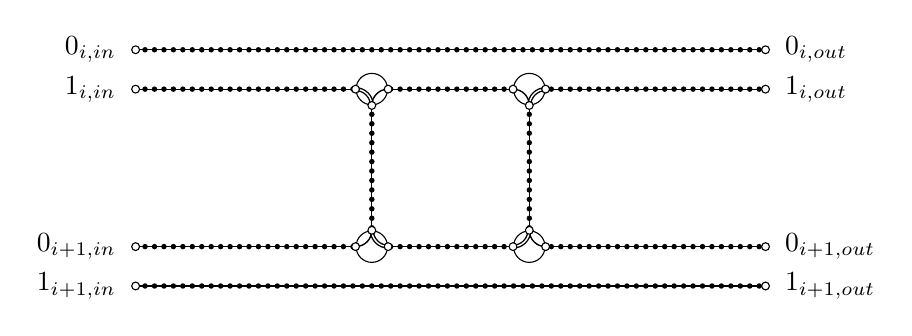
\begin{tikzpicture}[
  scale=2,
  split/.style={circle,draw=black,fill=white,
    inner sep=0pt, minimum size= 4mm},
  attach/.style={circle,draw=black,fill=white,
    inner sep=1pt, minimum size=0},
  vert/.style={circle,fill=black,inner sep=.7pt,minimum size=0}]

  \foreach \x in {0,.06,...,4}{
  \foreach \y in {.25, .5, 1.5, 1.75}{
    \node at (\x,\y) [vert] {};
  }}
  
  \foreach \x in {1.5,2.5}{
  \foreach \y in {.5,.56,...,1.5}{
    \node at (\x,\y) [vert]{};
  }}

  \draw (0,.25) node[label=left:$1_{i+1,\text{in}}$] {} 
     -- (4,.25) node[label=right:$1_{i+1,\text{out}}$] {};

  \node (s1) at (1.5,.5) [split] {};
  \node (s2) at (2.5,.5) [split] {};
  \node (s3) at (1.5,1.5) [split] {};
  \node (s4) at (2.5,1.5) [split] {};

  \draw (0,1.75) node[label=left:$0_{i,\text{in}}$] {}
     -- (4,1.75) node[label=right:$0_{i,\text{out}}$] {};

  \draw (0,.5) node[label=left:$0_{i+1,\text{in}}$] {}
     -- (s1.west);
  \draw (0,1.5) node[label=left:$1_{i,\text{in}}$] {}
     -- (s3.west);

  \draw (s4.east) -- (4,1.5) node[label=right:$1_{i,\text{out}}$]{};
  \draw (s2.east) -- (4,0.5) node[label=right:$0_{i+1,\text{out}}$]{};

  \draw (s1.east) -- (s2.west);
  \draw (s3.east) -- (s4.west);
  \draw (s1.north) -- (s3.south);
  \draw (s2.north) -- (s4.south);

  \draw (s1.west) to[out=0,in=-90] (s1.north)[line width=.5pt];
  \draw (s1.east) to[out=-180,in=-90] (s1.north) [line width =1.5pt];
  \draw (s1.east) to[out=-180,in=-90] (s1.north) [white,line width=.5pt];

  \draw (s2.east) to[out=-180,in=-90] (s2.north)[line width=.5pt];
  \draw (s2.west) to[out=0,in=-90] (s2.north)[line width=1.5pt];  
  \draw (s2.west) to[out=0,in=-90] (s2.north)[white,line width=.5pt];

  \draw (s3.east) to[out=-180,in=90] (s3.south)[line width=.5pt];
  \draw (s3.west) to[out=0,in=90] (s3.south)[line width=1.5pt];
  \draw (s3.west) to[out=0,in=90] (s3.south)[white,line width=.5pt];

  \draw (s4.west) to[out=0,in=90] (s4.south)[line width=.5pt];
  \draw (s4.east) to[out=-180,in=90] (s4.south)[line width=1.5pt];
  \draw (s4.east) to[out=-180,in=90] (s4.south)[white,line width=.5pt];

  \foreach \n in {s1, s2, s3, s4}{
    \node at (\n.west) [attach]{};
    \node at (\n.east) [attach]{};
  }
  
  \node at (s1.north) [attach]{};
  \node at (s2.north) [attach]{};
  \node at (s3.south) [attach]{};
  \node at (s4.south) [attach]{};
  
  \foreach \x in {0,4}{
  \foreach \y in {.25, .5, 1.5, 1.75}{
    \node at (\x,\y) [attach]{};
  }}
\end{tikzpicture}   
\caption[Planar entangling gate]{The planar entangling gate between adjacent encoded qubits $i$ and $i+1$. This graph implements the unitary $\XX_{i+1} (\CD)^2_{i,i+1} \XX_{i+1}$.}
\label{fig:PlanCPGate}
\end{figure}

\subsection{Distinguishable particles}

So far we have focused on the case of indistinguishable particles.  However, we can also perform universal quantum computation with distinguishable particles, provided the interaction has an appropriate form.

For distinguishable particles we will use use the same encoding of qubits as before, except that now each qubit is associated with a specific particle (e.g., computational qubit 1 is associated with particle 1). We have from \lem{MP_u_single_qubit_encoded_computation} that the single particle evolutions do not depend on the symmetries of the particles, and thus we need only examine the implementation of the $\CD$ gate to see how our construction must be modified. In this section we show that with a simple nearest-neighbor interaction we can make our scheme work for distinguishable particles by carefully choosing the strength of the interaction term in the Hamiltonian, but with no other modifications.

When two indistinguishable particles of momenta $k_1$ and $k_2$ scatter on an infinite path, there is no distinction between the final state where the particles reflect off of each other (exchanging momenta) and where the particles transmit through one another. Thus, after scattering, the global phase of the wave function is multiplied by a factor $T\pm R$, the sum of the amplitude to transmit and the amplitude to reflect (or the difference if the particles are fermions). For any interaction potential, $|T\pm R|=1$, and in most cases the applied phase is nontrivial and can be used for universal computation within our scheme. 

In contrast, when two \textit{distinguishable} particles of momenta $k_1$ and $k_2$ scatter on an infinite path, there are two distinct outgoing states:  one corresponding to the case where the two particles reflect and one where the particles transmit.  We circumvent this potential problem by choosing the interaction strength so that the transmission probability for two-particle scattering at momenta $k_1$ and $k_1$ is $1$ (forcing $R=0$), yet $T\neq 1$ (so that $T$ is a nontrivial phase). With such a choice, the graph implementing the $\CD$ gates preserves our encoding of qubits. In other words, if encoded qubit 1 is associated with particle 1 before applying the gate, then it is still associated with particle 1 after applying the gate (and similarly for the second qubit involved in the gate). We can then use the same graph as before to implement the controlled phase gate between encoded qubits.

Consider the nearest-neighbor Hamiltonian with $\mathcal{U}{1}(x,y) = \mathcal{U}_{1}xy$. For two particles on an infinite path, this is \eq{two_part_H_rs} with $\mathcal{V}(|r|)=U\delta_{|r|,1}$. The reflection coefficient $R(k_1,k_2)$  for $k_1=-\frac{\pi}{4}$ and $p_2 = \frac{\pi}{2}$ is
\[
  R\left(-\frac{\pi}{4},\frac{\pi}{2}\right) =\frac{-2U_{1}^{1,1}\left(\sqrt{2}+(\sqrt{2}-1)\mathcal{U}_{1}^{1,1}\right)}{(\sqrt{2} - 2)(1+i) (\mathcal{U}_{1}^{1,1})^2 - 4 \mathcal{U}_{1}^{1,1} + 2 i (\sqrt{2} + 2)}.
\]

Our goal is to choose $\mathcal{U}_{1}^{1,1}$ so that $R=0$ and $T$ is a nontrivial phase. The values of $\mathcal{U}_{1}^{1,1}$ that set $R=0$ are  $\mathcal{U}_{1}^{1,1} = 0$ or $\mathcal{U}_{1}^{1,1} = -2 - \sqrt{2}$.  The solution $\mathcal{U}_{1}^{1,1} = 0$ corresponds to no interaction and the trivial phase $T = 1$ which is not sufficient for universal computation within our scheme. Choosing $\mathcal{U}_{1}^{1,1}=-2-\sqrt{2}$ sets $T= i$ which allows us to perform a CP gate. 

We expect that other types of multi-particle quantum walk with distinguishable particles can also be used for universal computation. However, unlike in the case of indistinguishable particles, the interaction term may have to be tuned to satisfy the conditions $R=0$ and $T\neq1$  as was the case here.  For some interactions, it may not be possible to satisfy these two requirements.  For example, for a model where interactions only occur when particles occupy the same site (such as in the Bose-Hubbard model) we have $1+R = T$ for all momenta, so the transmission amplitude is trivial whenever $R=0$.

Note that it may be possible to implement an entangling two-qubit gate in other ways.  For example, some interactions may allow two-particle scattering with $T=0$ and $R=i$, in which case the graph shown in \fig{PlanCPGate} preserves the encoding of qubits and implements such a gate.

\section{Conclusions and open problems}

Using scattering theory for one and two-qubit interactions on a graph, we were able to encode $n$ qubits in the location of $n$-particles on a polynomial sized graph.  We then used our bounds on the scattering behavior for these small number of particles to understand the $n$-particle evolution.  

Note that we have already improved known results in this construction, as our error bounds are nearly a quadratic improvement.  However, the resulting bounds are still rather large; if we could improve these bounds in any manner, either by changing our construction or decreasing the error from scattering events, this would be a nice result.

\biblio{}

\end{document}